\documentclass[a4paper,12pt]{report}

% Кодировка и локализация
\usepackage{cmap} % Поддержка поиска и копирования русского текста в PDF
\usepackage[T2A]{fontenc}
\usepackage[utf8]{inputenc}
\usepackage[english,russian]{babel}

% Поля страниц по ГОСТ 7.32 (левое 30 мм, правое 15 мм, верхнее 20 мм, нижнее 20 мм)
\usepackage[left=3.0cm, right=1.5cm, top=2.0cm, bottom=2.0cm]{geometry}

% Полуторный интервал
\usepackage{setspace}
\onehalfspacing

% Абзацный отступ по ГОСТ (1.25 см)
\parindent=1.25cm
\parskip=0pt
\emergencystretch 3em % Предотвращение выхода текста за границы полей (overfull \hbox)

% Пакеты для математики
\usepackage{amsmath,amsfonts,amssymb,amsthm,mathtools}
\usepackage{icomma} % Умная запятая для десятичных дробей

% Пакеты для таблиц и графики
\usepackage{multirow}
\usepackage{graphicx}
\usepackage{float}
\usepackage{caption}

% Номера страниц вверху по центру или внизу по центру (по ГОСТ обычно внизу по центру или вверху по центру)
\pagestyle{plain}

% Пакет для определения последней страницы
\usepackage{lastpage}

% Вспомогательная команда для рисования плейсхолдеров рисунков
\newcommand{\rect}{%
    \begin{center}
        \fbox{\parbox[c][5cm][c]{10cm}{\centering\textit{Иллюстрация (график)}} }
    \end{center}
}

% Настройка гиперссылок
\usepackage[unicode,colorlinks=true,allcolors=blue,pdftex]{hyperref}

\begin{document}

% 1. Титульный лист
% \begin{center}
    \footnotesize{ФЕДЕРАЛЬНОЕ ГОСУДАРСТВЕННОЕ АВТОНОМНОЕ ОБРАЗОВАТЕЛЬНОЕ УЧРЕЖДЕНИЕ ВЫСШЕГО ОБРАЗОВАНИЯ}\\ 
    \footnotesize{МОСКОВСКИЙ ФИЗИКО-ТЕХНИЧЕСКИЙ ИНСТИТУТ\\(НАЦИОНАЛЬНЫЙ ИССЛЕДОВАТЕЛЬСКИЙ УНИВЕРСИТЕТ)}\\ 
    \footnotesize{ФАКУЛЬТЕТ ФИЗИКИ И ИССЛЕДОВАНИЙ ИМЕНИ ЛАНДАУ\\}
\end{center}

\vfill

\begin{figure}[H]
    \centering
    \includegraphics*[width=8cm,height=5cm,keepaspectratio]{image0.png}
\end{figure}

\vfill

\begin{center}
    \large{\textbf{ВЫПУСКНАЯ КВАЛИФИКАЦИОННАЯ РАБОТА БАКАЛАВРА}\\[0.4cm]
    \textbf{Математическое моделирование акустических волноводов на основе уравнения Вебстера и метода матриц длинных линий}}
\end{center}

\vfill

\begin{flushright}
    \begin{minipage}{0.55\textwidth}
        \textbf{Выполнил:}\\
        студент группы Б02-212\\
        Ерыкалкин Георгий Олегович\\[0.4cm]
        \textbf{Научный руководитель:}\\
        \textit{Петров Петр Петрович}\\
        доктор физ.-мат. наук, профессор\\[0.4cm]
        \textbf{Рецензент:}\\
        \textit{Сидоров Сидор Сидорович}\\
        кандидат физ.-мат. наук
    \end{minipage}
\end{flushright}

\vfill

\begin{center}
    Москва, 2026 г.
\end{center}
\thispagestyle{empty}
\newpage


% 2. Аннотация / Реферат
\chapter*{Реферат}
\addcontentsline{toc}{chapter}{Реферат}

Выпускная квалификационная работа бакалавра содержит \pageref{LastPage} страниц, \ref{fig_count} рисунков, \ref{tab_count} таблиц, \ref{ref_count} источников.

\textbf{Ключевые слова:} уравнение Вебстера, нейросетевые операторы, оператор Фурье (FNO), DeepONet, Mamba, сверточная сеть UNet, прямая и обратная задачи волноводной акустики.

\textbf{Объект исследования:} одномерные акустические волноводы переменного сечения и процессы распространения звуковых волн в них.

\textbf{Цель работы:} исследование и сравнительный анализ нейросетевых архитектур для решения прямой и обратной задач в одномерной акустике волноводов переменного сечения: быстрого предсказания спектрального отклика по геометрическому профилю и восстановления геометрического профиля по спектральному отклику.

В ходе работы был реализован набор численных решателей прямой задачи (TMM, ARMA, TLM), использованный для генерации данных, верификации результатов и сравнения с нейросетевыми моделями. Реализованы и обучены нейросетевые аппроксиматоры прямой задачи, включая MLP, FNO, DeepONet, Mamba Operator и ряд модификаций DeepONet. Проведено исследование влияния различных архитектурных решений в DeepONet, включая механизмы Mamba, SIREN, FiLM, Attention Fusion, а также динамические и деформируемые свертки. Для обратной задачи восстановления геометрии по спектральному отклику сопоставлены оптимизационные и нейросетевые подходы, включая градиентную оптимизацию, метод Метрополиса и специализированную сверточную модель UNet, обученную на двумерных пространственно-спектральных картах входа $[H, f, x]$.


% 3. Оглавление
\tableofcontents
\newpage

% 4. Введение
\chapter*{Введение}
\addcontentsline{toc}{chapter}{Введение}

\textbf{Актуальность темы.} Моделирование распространения звуковых волн в одномерных волноводах переменного сечения представляет собой классическую задачу технической акустики, которая находит широкое применение во многих прикладных областях. К ним относятся акустика музыкаческих инструментов (в частности, духовых рупоров), проектирование акустических систем и волноводных концентраторов, а также моделирование речевого тракта человека для задач синтеза речи. Одномерное приближение на основе уравнения Вебстера позволяет существенно сократить вычислительные затраты по сравнению с полномерным трехмерным моделированием уравнений Навье--Стокса или Гельмгольца при сохранении высокой физической точности в области низких и средних частот.

Существующие подходы к численному расчету одномерного акустического поля делятся на методы матриц передачи (TMM) для кусочно-постоянной или кусочно-конической аппроксимации геометрии, метод матриц длинных линий (Transmission Line Matrix, TLM), а также авторегрессионные схемы (ARMA), позволяющие свести расчет к быстрым полиномиальным операциям. Каждый из этих подходов обладает уникальным балансом вычислительной сложности, точности и возможностей расширения. В связи с этим актуальной задачей является проведение систематического исследования и сравнительного анализа данных методов на репрезентативном наборе тестовых геометрий.

\textbf{Цель работы} --- разработка кроссплатформенного программного комплекса для численного моделирования акустических полей в волноводах переменного сечения и проведение комплексного сравнительного анализа методов TMM (цилиндрического и конического), авторегрессионного моделирования ARMA и метода TLM по критериям точности, сходимости и времени выполнения.

Для достижения поставленной цели необходимо решить следующие \textbf{задачи}:
\begin{enumerate}
    \item Изучить теоретические основы одномерной волновой акустики и математический аппарат уравнения Вебстера.
    \item Реализовать методы расчета передаточных матриц для цилиндрических и конических сегментов (TMM).
    \item Разработать эффективный решатель на основе авторегрессионного скользящего среднего (ARMA) для ускорения частотных расчетов.
    \item Разработать эффективный решатель на основе метода матриц длинных линий (TLM) на языке C++ с возможностью интеграции в Python-окружение.
    \item Провести серию численных экспериментов по верификации реализованных решателей на регулярных и сложных геометриях волноводов.
    \item Выполнить комплексный сравнительный анализ вычислительной эффективности и точности реализованных методов.
\end{enumerate}

\textbf{Научная новизна} работы заключается в систематическом сравнении классических частотных методов TMM с авторегрессионным подходом ARMA в z-области и временным методом TLM для широкого класса гладких, кусочно-непрерывных и резонансных геометрий волноводов.




% 5. Основная часть (Главы)
\chapter{Математические модели акустических волноводов}
\label{ch:theory}

В данной главе рассматриваются теоретические аспекты распространения звуковых волн в волноводах переменного сечения в одномерном приближении. Дается вывод уравнения Вебстера и приводится описание метода матриц передачи (TMM) для цилиндрической и конической аппроксимаций геометрии.

\section{Уравнение рупора Вебстера}
\label{sec:webster}

Распространение звуковых волн в жесткостенном канале переменного поперечного сечения $A(x)$ описывается классическим волновым уравнением рупора Вебстера (Webster horn equation)~\cite{webster1919}. Это одномерное уравнение является хорошим приближением для волн, длина которых существенно превышает поперечные размеры канала (то есть для плоских волн).

Математическая формулировка уравнения Вебстера для акустического давления $p(x, t)$ имеет следующий вид:
\begin{equation}
    \frac{1}{A(x)} \frac{\partial}{\partial x} \left( A(x) \frac{\partial p(x, t)}{\partial x} \right) - \frac{1}{c^2} \frac{\partial^2 p(x, t)}{\partial t^2} = 0,
    \label{eq:webster_time}
\end{equation}
где $x$ --- координата вдоль оси волновода, $t$ --- время, $c$ --- скорость звука в среде.

Для гармонических волн с временной зависимостью $e^{j\omega t}$ уравнение Вебстера во временной области переходит в уравнение в частотной области:
\begin{equation}
    \frac{d^2 P(x, \omega)}{dx^2} + \frac{1}{A(x)} \frac{dA(x)}{dx} \frac{dP(x, \omega)}{dx} + k^2 P(x, \omega) = 0,
    \label{eq:webster_freq}
\end{equation}
где $P(x, \omega)$ --- комплексная амплитуда акустического давления, $k = \omega / c$ --- волновое число, $\omega = 2\pi f$ --- круговая частота.

Если ввести вспомогательную функцию $\psi(x) = P(x) \sqrt{A(x)}$, то уравнение~\eqref{eq:webster_freq} может быть преобразовано к одномерному уравнению Шредингера:
\begin{equation}
    \frac{d^2 \psi(x)}{dx^2} + [k^2 - V(x)] \psi(x) = 0,
\end{equation}
где $V(x) = \frac{1}{2 A} \frac{d^2 A}{dx^2} - \frac{1}{4 A^2} \left(\frac{dA}{dx}\right)^2$ представляет собой так называемый «потенциал рупора».

\section{Метод матриц передачи (TMM)}
\label{sec:tmm}

Метод матриц передачи (Transfer Matrix Method, TMM) основан на представлении сложного акустического волновода в виде каскадного соединения более простых элементов (сегментов), для каждого из которых известно точное аналитическое решение. Переменными состояния на границах сегментов являются акустическое давление $P$ и объемная колебательная скорость $U$.

Для любого акустического элемента связь между входными ($P_{in}, U_{in}$) и выходными ($P_{out}, U_{out}$) величинами записывается через матрицу передачи $T$ размера $2 \times 2$:
\begin{equation}
    \begin{pmatrix} P_{in} \\ U_{in} \end{pmatrix} = 
    \begin{pmatrix} T_{11} & T_{12} \\ T_{21} & T_{22} \end{pmatrix}
    \begin{pmatrix} P_{out} \\ U_{out} \end{pmatrix}.
\end{equation}

При каскадном соединении $N$ сегментов общая матрица передачи всей системы равна произведению матриц передачи отдельных сегментов:
\begin{equation}
    T_{total} = T_1 \cdot T_2 \cdot \dots \cdot T_N.
\end{equation}

\subsection{Цилиндрическая аппроксимация геометрии}
Наиболее простым способом дискретизации является разбиение волновода на $N$ цилиндрических сегментов постоянного сечения. Для цилиндра длиной $l$ и площадью поперечного сечения $A$ элементы матрицы передачи имеют вид~\cite{chiba2006}:
\begin{equation}
    T_{cyl} = \begin{pmatrix} 
        \cos(kl) & j Z_0 \sin(kl) \\ 
        \frac{j}{Z_0} \sin(kl) & \cos(kl) 
    \end{pmatrix},
\end{equation}
где $Z_0 = \frac{\rho_0 c}{A}$ --- характеристический волновой импеданс цилиндрического волновода, $\rho_0$ --- плотность среды.

\subsection{Коническая аппроксимация геометрии}
Коническая аппроксимация волновода обеспечивает более точное представление геометрии с непрерывным изменением площади. Для конического сегмента с площадями на входе $A_{in}$ (радиус $r_{in}$) и выходе $A_{out}$ (радиус $r_{out}$) и длиной $l$ элементы матрицы передачи выражаются через сферические функции:
\begin{equation}
    T_{cone} = \begin{pmatrix}
        \frac{r_{out}}{r_{in}} \cos(kl) - \frac{1}{k r_{in}} \sin(kl) & j \frac{\rho_0 c}{S_{in}} \frac{r_{out}}{r_{in}} \sin(kl) \\
        \dots & \dots
    \end{pmatrix}.
\end{equation}
Использование конических сегментов позволяет снизить число необходимых элементов разбиения для достижения той же точности по сравнению с чисто цилиндрической аппроксимацией.

\chapter{Решение прямой задачи}
\label{ch:direct_problem}

В данной главе рассматривается решение прямой задачи акустического моделирования — быстрое прогнозирование передаточной функции волновода по известному распределению площади его поперечного сечения с помощью нейросетевых моделей. Основная цель данного этапа состоит в замене ресурсоемких численных решателей, описанных в главе 1, на быстрые дифференцируемые аппроксиматоры, способные рассчитывать спектральный отклик за доли миллисекунды.

\section{Постановка задачи аппроксимации}
\label{sec:approximation_statement}

Математически прямая задача формулируется как построение отображения $\mathcal{F}_{\theta}$, параметризованного весами нейросети $\theta$:
\begin{equation}
    \mathcal{F}_{\theta} : \mathbf{a} \longmapsto \mathbf{h}_{\mathrm{dB}},
\end{equation}
где вектор входа $\mathbf{a} = [A_1, A_2, \dots, A_{N_s}]^T \in \mathbb{R}^{N_s}$ представляет собой дискретный профиль площадей поперечного сечения волновода вдоль его продольной оси в $N_s$ узлах пространственной сетки. Вектор выхода $\mathbf{h}_{\mathrm{dB}} = [H_{\mathrm{dB}}(f_1), H_{\mathrm{dB}}(f_2), \dots, H_{\mathrm{dB}}(f_{N_f})]^T \in \mathbb{R}^{N_f}$ содержит амплитуду передаточной функции в децибельной шкале, вычисленную на заданной сетке частот $\{f_i\}_{i=1}^{N_f}$ в диапазоне $[f_{\min}, f_{\max}]$.

В качестве обучающей выборки используется датасет, сгенерированный с помощью эталонного конического TMM-решателя:
\begin{equation}
    \mathcal{D} = \left\{ \left( \mathbf{a}^{(k)}, \mathbf{h}_{\mathrm{dB}}^{(k)} \right) \right\}_{k=1}^{N_{\mathrm{samples}}}.
\end{equation}

\section{Комбинированный функционал потерь}
\label{sec:loss_function}

Стандартные метрики обучения, такие как среднеквадратичная ошибка (MSE) или средняя абсолютная ошибка (MAE) на шкале децибел, не в полной мере учитывают физические особенности резонансного акустического спектра. Для повышения точности аппроксимации формы резонансов (формант) в работе использовался универсальный многокомпонентный функционал потерь $L_{\text{total}}$, объединяющий амплитудные, относительные, производные и пиковые характеристики спектров:
\begin{equation}
    L_{\text{total}} = w_{\text{dB}} L_{\text{dB}} + w_{\text{mag}} L_{\text{mag}} + w_{\text{deriv}} L_{\text{deriv}} + w_{\text{peak}} L_{\text{peak}} + w_{\text{level}} L_{\text{level}},
\end{equation}
где $w_{\text{dB}}, w_{\text{mag}}, w_{\text{deriv}}, w_{\text{peak}}, w_{\text{level}}$ — весовые коэффициенты. В основных экспериментах использовались компоненты ошибки в децибелах, относительной ошибки линейной амплитуды, ошибки производной и ошибки уровня доминирующего пика; компоненту soft-argmax положения пика можно включать отдельно через ненулевой вес $w_{\text{peak}}$. Идея совместного использования линейных и логарифмических спектральных расстояний заимствована из дифференцируемых спектральных лоссов, применяемых в моделях DDSP~\cite{engel2020ddsp}.

Математически компоненты функционала потерь определяются следующим образом:

\begin{enumerate}
    \item \textbf{Ошибка логарифмической АЧХ ($L_{\text{dB}}$)}
    Для глобального совмещения формы спектра на логарифмической шкале децибел используется функция Smooth L1 с нормирующим коэффициентом $S_{\text{dB}} = 10$ для стабилизации масштаба градиентов:
    \begin{equation}
        L_{\text{dB}} = \frac{1}{N_f} \sum_{i=1}^{N_f} \text{Smooth}_{L_1} \left( \frac{\widehat{H}_{\text{dB}}(f_i) - H_{\text{dB}}(f_i)}{S_{\text{dB}}} \right),
    \end{equation}
    где $H_{\text{dB}}$ — эталонный спектр, полученный опорным численным решателем, $\widehat{H}_{\text{dB}}$ — предсказание модели, а $\text{Smooth}_{L_1}(x)$ задается как:
    \begin{equation}
        \text{Smooth}_{L_1}(x) = \begin{cases} 
            0.5 x^2, & |x| < 1, \\
            |x| - 0.5, & |x| \ge 1.
        \end{cases}
    \end{equation}

    \item \textbf{Относительная ошибка линейной амплитуды ($L_{\text{mag}}$)}
    Для акцентирования внимания модели на областях высоких резонансных пиков (где амплитуда велика) вводится нормированное $L_2$-расстояние в линейном масштабе:
    \begin{equation}
        L_{\text{mag}} = \frac{\sqrt{\sum_{i=1}^{N_f} \left(\widehat{H}(f_i) - H(f_i)\right)^2}}{\sqrt{\sum_{i=1}^{N_f} H(f_i)^2} + \varepsilon_0},
    \end{equation}
    где $H(f_i) = 10^{H_{\text{dB}}(f_i)/20}$, $\widehat{H}(f_i) = 10^{\widehat{H}_{\text{dB}}(f_i)/20}$ — линейные амплитуды передаточных функций, а $\varepsilon_0 = 10^{-8}$ исключает деление на ноль.

    \item \textbf{Ошибка по производной АЧХ по частоте ($L_{\text{deriv}}$)}
    Сглаженность передаточных функций и наклон склонов резонансных пиков контролируются разностью производных по частоте с масштабом $S_{\text{deriv}} = 0.01$:
    \begin{equation}
        L_{\text{deriv}} = \frac{1}{N_f - 1} \sum_{i=1}^{N_f - 1} \text{Smooth}_{L_1} \left( \frac{\Delta \widehat{H}_{\text{dB}}(f_i) - \Delta H_{\text{dB}}(f_i)}{S_{\text{deriv}} \cdot \Delta f_i} \right),
    \end{equation}
    где $\Delta H_{\text{dB}}(f_i) = H_{\text{dB}}(f_{i+1}) - H_{\text{dB}}(f_i)$, $\Delta \widehat{H}_{\text{dB}}(f_i) = \widehat{H}_{\text{dB}}(f_{i+1}) - \widehat{H}_{\text{dB}}(f_i)$, а $\Delta f_i = f_{i+1} - f_i$ — шаг частотной сетки.

    \item \textbf{Ошибка положения доминирующего резонансного пика ($L_{\text{peak}}$)}
    Для точного совпадения частот главных резонансов вводится дифференцируемое приближение положения пика через оператор soft-argmax:
    \begin{equation}
        L_{\text{peak}} = \frac{|f_{\text{peak}} - \widehat{f_{\text{peak}}}|}{f_{N_f} - f_1},
    \end{equation}
    где взвешенная частота пика $f_{\text{peak}}$ (и аналогично для $\widehat{f_{\text{peak}}}$) находится по распределению softmax:
    \begin{equation}
        f_{\text{peak}} = \sum_{i=1}^{N_f} f_i \cdot w_i, \quad w_i = \frac{\exp\left(H_{\text{dB}}(f_i)/T\right)}{\sum_{j=1}^{N_f} \exp\left(H_{\text{dB}}(f_j)/T\right)},
    \end{equation}
    где $T = 3.0$ дБ — температурный параметр. Данный подход к плавной частотной аппроксимации пиковых значений заимствует идею взвешенного суб-бинового усреднения, успешно примененного в алгоритме CREPE для высокоточного трекинга частот~\cite{kim2018crepe}.

    \item \textbf{Ошибка уровня доминирующего пика ($L_{\text{level}}$)}
    В основных экспериментах дополнительно штрафовалось несовпадение амплитуды доминирующего резонансного пика:
    \begin{equation}
        L_{\text{level}} = \left| \max_i \widehat{H}_{\text{dB}}(f_i) - \max_i H_{\text{dB}}(f_i) \right|.
    \end{equation}
    Эта компонента напрямую контролирует высоту наиболее выраженного резонанса и не требует дифференцируемого поиска его частоты.
\end{enumerate}

\section{Архитектуры нейросетевых моделей}
\label{sec:architectures}

В данной работе для решения прямой задачи исследуются четыре базовые нейросетевые архитектуры различного класса: базовый многослойный перцептрон (MLP), Фурье-нейросетевой оператор (FNO), нейронная сеть оператора DeepONet и нейросетевой оператор Mamba (Mamba Operator).

\subsection{Многослойный перцептрон (MLP)}
\label{subsec:mlp}

Многослойный перцептрон (Multilayer Perceptron, MLP) используется в качестве базовой модели. Входной вектор профиля сечений преобразуется полносвязной структурой, где каждый канал обрабатывается с нормализацией слоев LayerNorm и функцией активации GELU для ускорения градиентного спуска. В данной работе сеть имеет 4 скрытых полносвязных слоя размерностью $512$, а регуляризация осуществляется методом Dropout с коэффициентом $0.05$. Выходной линейный слой размерности $N_f$ формирует вектор предсказанной передаточной функции $\widehat{\mathbf{h}}_{\mathrm{dB}}$.

Преобразование на каждом скрытом слое $l \in [1, L_s]$ записывается в виде:
\begin{equation}
    \mathbf{z}^{(l)} = \operatorname{GELU} \left( \operatorname{LayerNorm} \left( \mathbf{W}^{(l)} \mathbf{z}^{(l-1)} + \mathbf{b}^{(l)} \right) \right),
\end{equation}
где $\mathbf{W}^{(l)}$ — веса слоя, $\mathbf{b}^{(l)}$ — вектор смещения, а $\mathbf{z}^{(0)} = \mathbf{a}$. Выход модели определяется как:
\begin{equation}
    \widehat{\mathbf{h}}_{\mathrm{dB}} = \mathbf{W}^{(L_s+1)} \mathbf{z}^{(L_s)} + \mathbf{b}^{(L_s+1)}.
\end{equation}

Благодаря своей простоте, модель MLP имеет высокую скорость вычислений, однако в ней отсутствует встроенное индуктивное смещение на локальность и трансляционную структуру пространственного профиля, характерное для сверточных и операторных архитектур.

\subsection{Модель с FNO-энкодером геометрии}
\label{subsec:fno}

В данной работе использовалась не классическая постановка FNO как прямого оператора ``поле-в-поле'', а гибридная архитектура с \emph{FNO-энкодером геометрии} и последующим \emph{частотно-условным декодером}. Спектральные слои FNO~\cite{li2020fourier} применялись только для извлечения глобальных признаков профиля канала, после чего предсказание значения $\widehat{H}(f)$ выполнялось отдельной декодирующей сетью, зависящей от частотного запроса. Поэтому далее для краткости данная модель обозначается как FNO, однако фактически она ближе к архитектуре ``FNO-based geometry encoder with a frequency-conditioned decoder''. Важно отметить, что в рассматриваемой основной постановке все каналы имели одинаковую физическую длину $L=1$ м, поэтому нормировка профиля по координате $x/L$ использовалась только как удобное приведение к общей сетке и не скрывала дополнительную вариативность по длине.

Схема работы FNO для решения прямой задачи выглядит следующим образом:
1. Входной профиль $\mathbf{a}(x)$ проецируется с помощью локальной полносвязной сети (лифтинга) в пространство с большим числом каналов $d_{\text{hidden}} = 96$.
2. Сигнал последовательно проходит через 4 Фурье-слоя. Каждый слой выполняет быстрое дискретное преобразование Фурье (FFT), фильтрует высокие частоты, оставляя лишь $N_{\text{modes}} = 32$ низших мод, умножает их на комплексную матрицу параметров $\mathbf{R}$, после чего выполняет обратное FFT. Параллельно применяется пространственная скип-связь (Skip Connection) через 1D-свертку:
\begin{equation}
    \mathbf{v}^{(l+1)}(x) = \sigma \left( \mathcal{F}^{-1} \left( \mathbf{R}^{(l)} \mathcal{F}(\mathbf{v}^{(l)}) \right)(x) + \mathbf{W}^{(l)} \mathbf{v}^{(l)}(x) \right),
\end{equation}
где $\mathcal{F}$ и $\mathcal{F}^{-1}$ — прямое и обратное FFT, $\mathbf{R}^{(l)}$ — обучаемые комплексные веса в спектральной области, $\mathbf{W}^{(l)}$ — сверточные веса в физическом пространстве, а $\sigma$ — нелинейность GELU.
3. Пространственная геометрия сжимается с помощью адаптивного пулинга (Adaptive Average Pooling) до $16$ элементов и преобразуется полносвязной геометрической головкой (Geometry Head) во временное латентное представление геометрии $\mathbf{v}_{\text{geom}} \in \mathbb{R}^{256}$.
4. Частотная координата $f$ линейно нормируется в диапазон $[0, 1]$ на фиксированном физическом интервале 50--5000 Гц (обозначим эту нормированную координату $\kappa$) и кодируется гармоническими признаками (гармонический эмбеддинг с $N_{\mathrm{bands}} = 8$ частотными полосами, дающий 17-мерный вектор), после чего преобразуется частотной головкой (Frequency Head) в вектор $\mathbf{v}_{\text{freq}} \in \mathbb{R}^{64}$. Поскольку в основном датасете длина канала не менялась, такая нормировка частоты была однозначной и не требовала явной подачи $L$ в модель.
5. Итоговый декодер объединяет латентное представление геометрии и код частотного запроса, формируя значение АЧХ $\widehat{H}_{\text{dB}}(f)$.

Таким образом, в реализованной архитектуре FNO не отображает входной профиль непосредственно в дискретизированное поле спектра на всей частотной сетке, как это часто делается в классических операторных постановках. Вместо этого FNO играет роль энкодера геометрии, а само значение передаточной функции вычисляется координатным декодером по паре ``латент геометрии -- частота''.

\subsection{Нейросеть оператора DeepONet}
\label{subsec:deeponet}

Архитектура DeepONet (Deep Operator Network)~\cite{lu2021learning} основана на разделении входа (функции профиля) и запроса (частотной координаты) на две независимые подсети. Как и в случае FNO, в основной серии экспериментов длина всех каналов была фиксирована и равна 1 м, поэтому нормировка профиля по $x/L$ не создавала неоднозначности, а отдельный признак длины в branch-вход не подавался.
\begin{itemize}
    \item \textbf{Ветвь (Branch Net)}: кодирует входную функцию геометрии $\mathbf{a}(x)$. Ветвь представляет собой 1D-сверточную сеть с $4$ остаточными блоками (Residual Blocks) с размером каналов $64$. Пространственный профиль сжимается пулингом до $16$ элементов и отображается полносвязным слоем в вектор коэффициентов разложения $\mathbf{b} \in \mathbb{R}^{p}$ размерностью $p = 128$.
    \item \textbf{Ствол (Trunk Net)}: кодирует координату запроса (частоту, линейно нормированную к диапазону $\kappa \in [0, 1]$ на фиксированном интервале 50--5000 Гц). Входная частота переводится в гармонический эмбеддинг с $N_{\mathrm{bands}} = 8$ частотными полосами по формуле:
    \begin{equation}
        \mathbf{v}_{\mathrm{embed}}(\kappa) = \left[ \kappa, \sin(\pi \kappa), \cos(\pi \kappa), \dots, \sin(\pi 2^7 \kappa), \cos(\pi 2^7 \kappa) \right]^T \in \mathbb{R}^{17}.
    \end{equation}.
    Полученный вектор пропускается через MLP с шириной слоев $128$. Ствол вычисляет набор базисных функций $\mathbf{t}(\kappa) \in \mathbb{R}^{p}$.
\end{itemize}

Выходное значение передаточной функции в точке $f$ определяется как скалярное произведение выходов ветви и ствола с добавлением обучаемого смещения:
\begin{equation}
    \widehat{H}_{\text{dB}}(f) = \frac{1}{\sqrt{p}} \sum_{j=1}^{p} b_j(\mathbf{a}) \cdot t_j(f) + b_0.
\end{equation}

DeepONet обладает высокой гибкостью, так как ствол обучается формировать оптимальные спектральные базисные функции (схожие с собственными модами резонатора), а ветвь определяет вклад каждой моды для конкретной геометрии. Подчеркнем, что приведенная реализация относится именно к случаю фиксированной длины канала. В экспериментах с варьированием длины такой параметр необходимо либо фиксировать заранее через пересчет геометрии и частотной оси, либо явно включать в частотный запрос и/или вход ветви.

\subsection{Нейросетевой оператор Mamba (Mamba Operator)}
\label{subsec:mamba_operator}

Нейросетевой оператор Mamba (Mamba Operator) основан на использовании блоков пространства состояний Mamba-2 для последовательной обработки геометрического профиля и частотной координаты. В отличие от архитектуры DeepONet, где ветвь и ствол сливаются на самом выходе, в Mamba Operator слияние происходит на более глубоком уровне с использованием механизма Feature-wise Linear Modulation (FiLM):
\begin{itemize}
    \item \textbf{Кодировщик геометрии (Geometry Token Encoder)}: преобразует пространственный профиль площадей $\mathbf{a}(x)$ с помощью 1D-сверточных слоев в последовательность геометрических токенов $\mathbf{v}_{\text{geom}} \in \mathbb{R}^{N_s \times d_{\text{model}}}$.
    \item \textbf{Кодировщик частоты (Frequency Token Encoder)}: проецирует частоту в латентное представление $\mathbf{v}_{\text{freq}} \in \mathbb{R}^{d_{\text{model}}}$.
\end{itemize}

Для каждой частоты геометрические токены модулируются аффинными параметрами $\gamma(\mathbf{v}_{\text{freq}})$ и $\beta(\mathbf{v}_{\text{freq}})$, вычисленными из частотного представления:
\begin{equation}
    \mathbf{z}_{\text{cond}} = \mathbf{v}_{\text{geom}} \odot (1 + \gamma) + \beta.
\end{equation}

Полученная модулированная последовательность обрабатывается в прямом и обратном направлениях по пространственной оси $x$ с помощью блоков двунаправленной Mamba-2 (\texttt{mamba\_forward} и \texttt{mamba\_backward}), что позволяет моделировать распространение волны вдоль волновода. Выходы блоков объединяются, и проекционная головка (Output Head) вычисляет итоговое значение передаточной функции $\widehat{H}_{\text{dB}}(f)$.

\section{Сравнение точности и скорости работы моделей}
\label{sec:comparison_results}

Обучение моделей MLP, FNO, DeepONet и Mamba Operator проводилось в режиме бесконечной динамической генерации случайных трубчатых геометрий на лету. В качестве функции потерь использовался комбинированный лосс $L_{\text{total}}$. Сравнение качества моделей проводилось на отложенной валидационной выборке.

Для количественной оценки качества аппроксимации передаточных функций на валидационной выборке использовались четыре основные метрики:
\begin{enumerate}
    \item \textbf{Средняя абсолютная ошибка (MAE)} в децибельной шкале по всему частотному диапазону:
    \begin{equation}
        \text{MAE} = \frac{1}{B \cdot N_f} \sum_{k=1}^B \sum_{i=1}^{N_f} \left| \widehat{H}_{\mathrm{dB}}^{(k)}(f_i) - H_{\mathrm{dB}}^{(k)}(f_i) \right|,
    \end{equation}
    где $B$ --- размер валидационной выборки, $N_f$ --- количество частот, $\widehat{H}_{\mathrm{dB}}$ и $H_{\mathrm{dB}}$ --- предсказанная и эталонная АЧХ соответственно.
    
    \item \textbf{Ошибка уровня доминирующего резонансного пика (Peak Level MAE)}:
    \begin{equation}
        \text{Peak\_MAE} = \frac{1}{B} \sum_{k=1}^B \left| \max_{i} \widehat{H}_{\mathrm{dB}}^{(k)}(f_i) - \max_{i} H_{\mathrm{dB}}^{(k)}(f_i) \right|.
    \end{equation}
    
    \item \textbf{Ошибка уровня доминирующего провала (Notch Level MAE)}:
    \begin{equation}
        \text{Notch\_MAE} = \frac{1}{B} \sum_{k=1}^B \left| \min_{i} \widehat{H}_{\mathrm{dB}}^{(k)}(f_i) - \min_{i} H_{\mathrm{dB}}^{(k)}(f_i) \right|.
    \end{equation}
    Данная метрика вычисляется исключительно в процессе валидации для оценки точности передачи глубоких антирезонансов и не входит в минимизируемый лосс $L_{\text{total}}$.
    
    \item \textbf{Относительная $L_2$-ошибка производной по частоте (Deriv Error)}:
    \begin{equation}
        \text{Deriv\_Error} = \frac{1}{B} \sum_{k=1}^B \frac{\left\| D_f \widehat{H}_{\mathrm{dB}}^{(k)} - D_f H_{\mathrm{dB}}^{(k)} \right\|_2}{\left\| D_f H_{\mathrm{dB}}^{(k)} \right\|_2 + \varepsilon_{\mathrm{eps}}},
    \end{equation}
    где $D_f H_i = \frac{H_{i+1} - H_i}{f_{i+1} - f_i}$ --- конечно-разностная производная по частотной координате, а $\varepsilon_{\mathrm{eps}} = 10^{-12}$. Эта метрика оценивает соответствие наклонов резонансных пиков и общую форму спектра.
\end{enumerate}

Для обоснования выбора комбинированной функции потерь $L_{\text{total}}$ было проведено обучение базовой модели MLP с использованием стандартной среднеквадратичной ошибки (MSE) в качестве функции потерь (модель MLP MSE baseline). Данная модель показала крайне низкую сходимость: наилучшее значение функции потерь на обучающей выборке составило $8.6561$, а на валидационной — $8.5690$. Это существенно хуже результатов аналогичной модели MLP, обученной с использованием комбинированной функции потерь $L_{\text{total}}$, что подтверждает необходимость включения дополнительных спектральных компонент, связанных с формой АЧХ, производной и уровнем доминирующего пика.

Подробное сравнение всех исследованных нейросетевых моделей — базовых конфигураций (MLP, FNO, DeepONet, Mamba Operator) и различных архитектурных модификаций оператора DeepONet — приведено в единой таблице~\ref{tab:modifications_comparison} в подразделе~\ref{subsec:modifications_comparison}.

Сравнение кривых сходимости функций потерь и изменения валидационного MAE в процессе обучения представлено на рис.~\ref{fig:loss_curves_comparison} и рис.~\ref{fig:metrics_curves_comparison} соответственно. Спектральное сравнение точности предсказания моделей для тестового образца приведено на общем рисунке~\ref{fig:all_spectrums} в конце раздела~\ref{sec:deeponet_modifications}.

\begin{figure}[H]
    \centering
    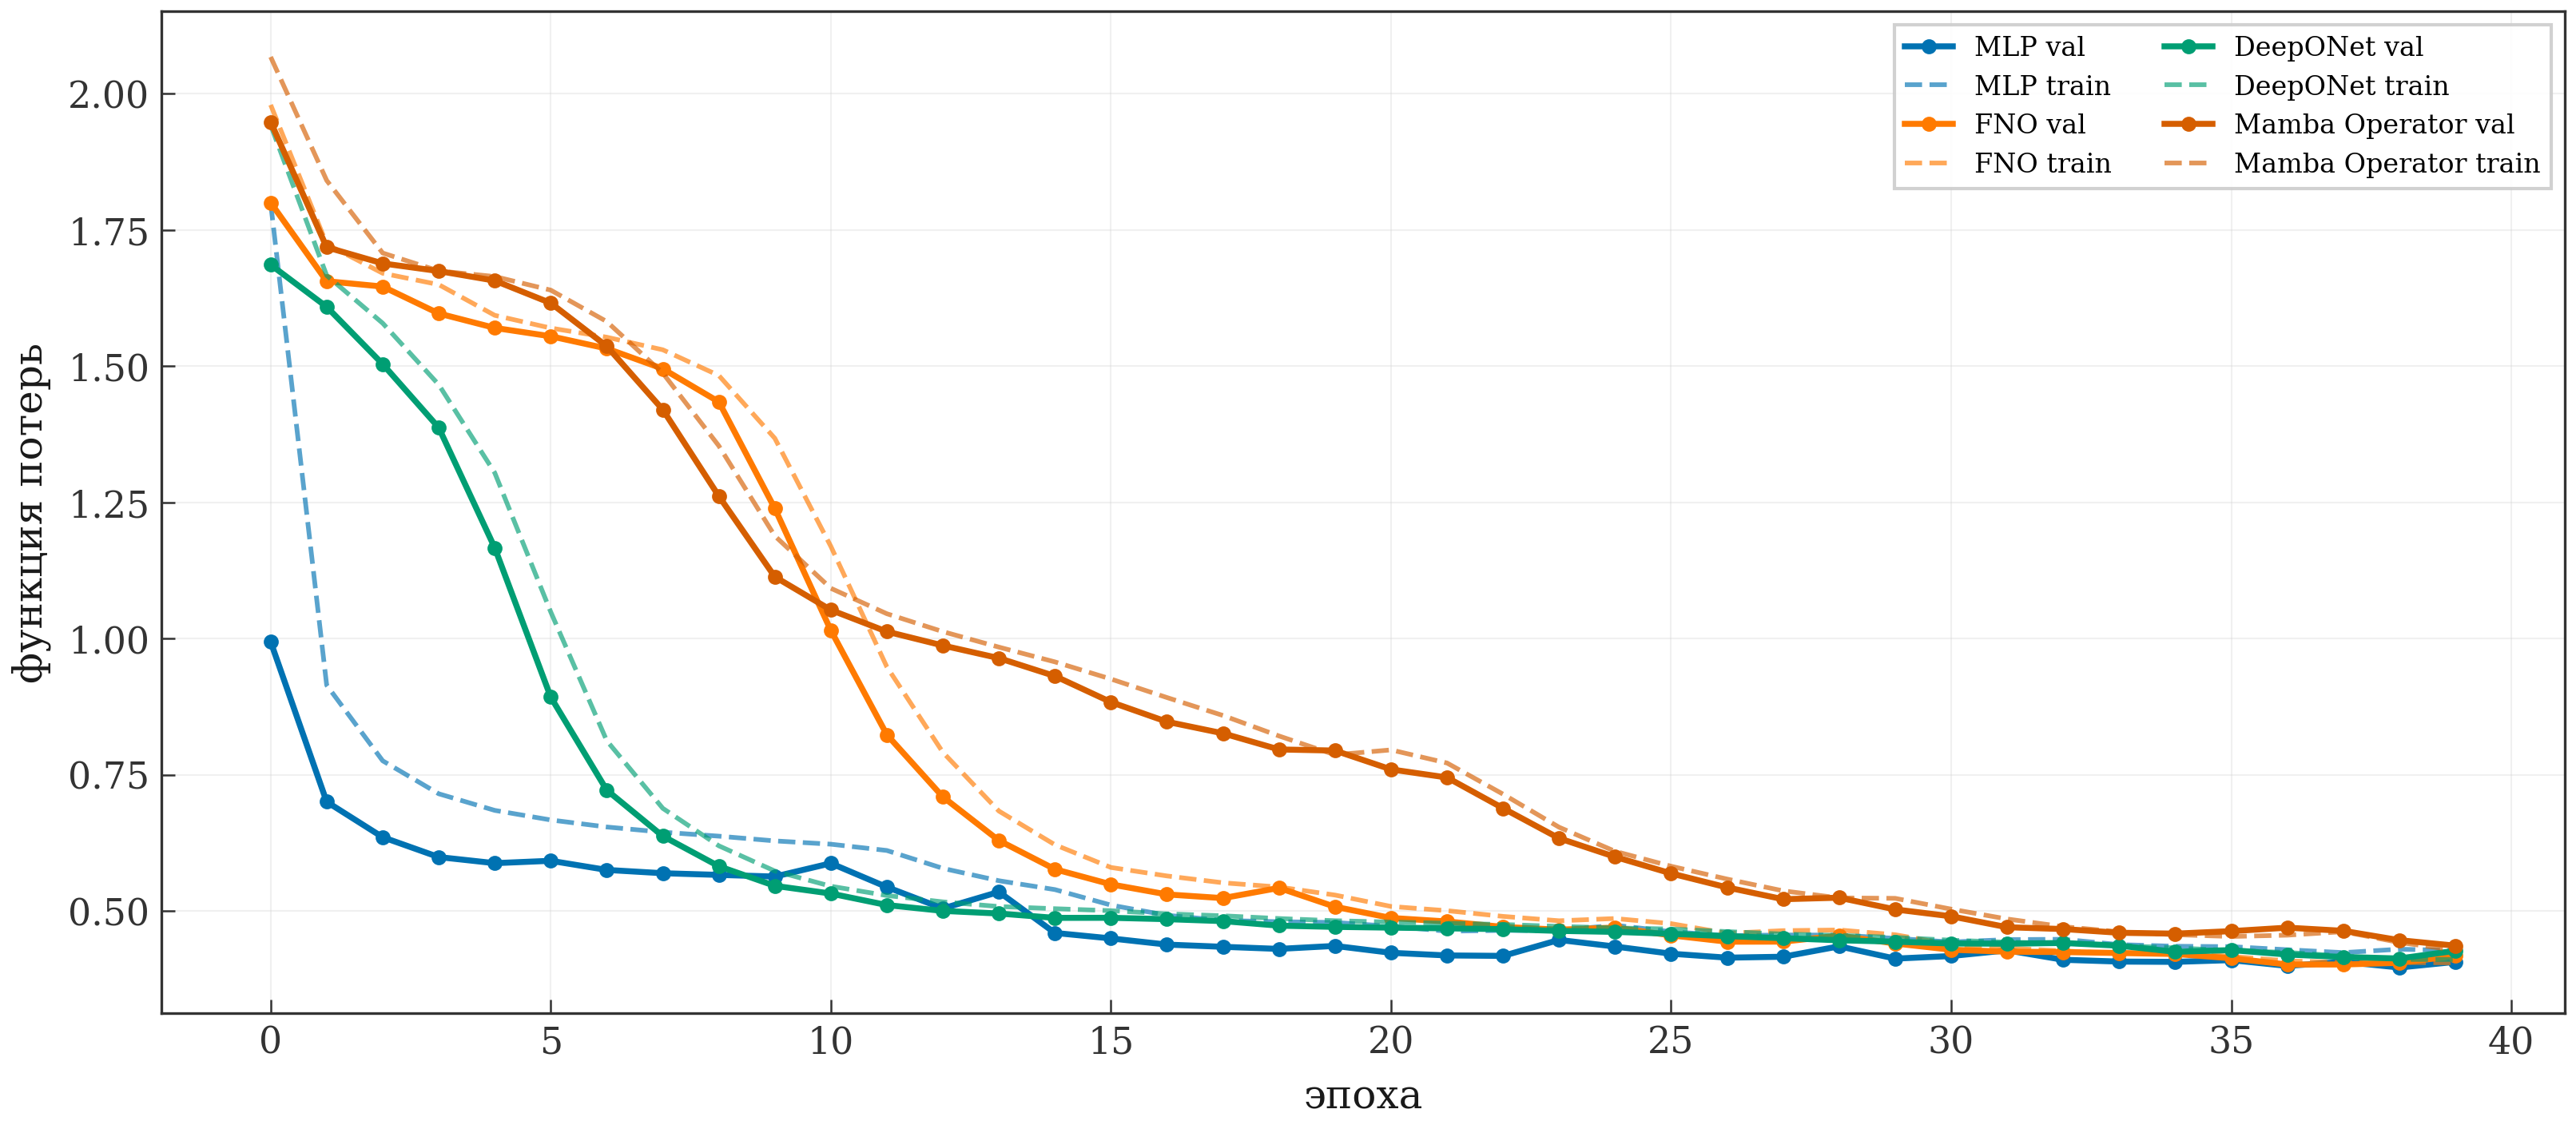
\includegraphics[width=0.95\textwidth]{images/функции_потерь_mlp_fno_deep_mamba.png}
    \caption{Сравнение сходимости функции потерь $L_{\text{total}}$ для базовых архитектур MLP, FNO, DeepONet и Mamba Operator.}
    \label{fig:loss_curves_comparison}
\end{figure}

\begin{figure}[H]
    \centering
    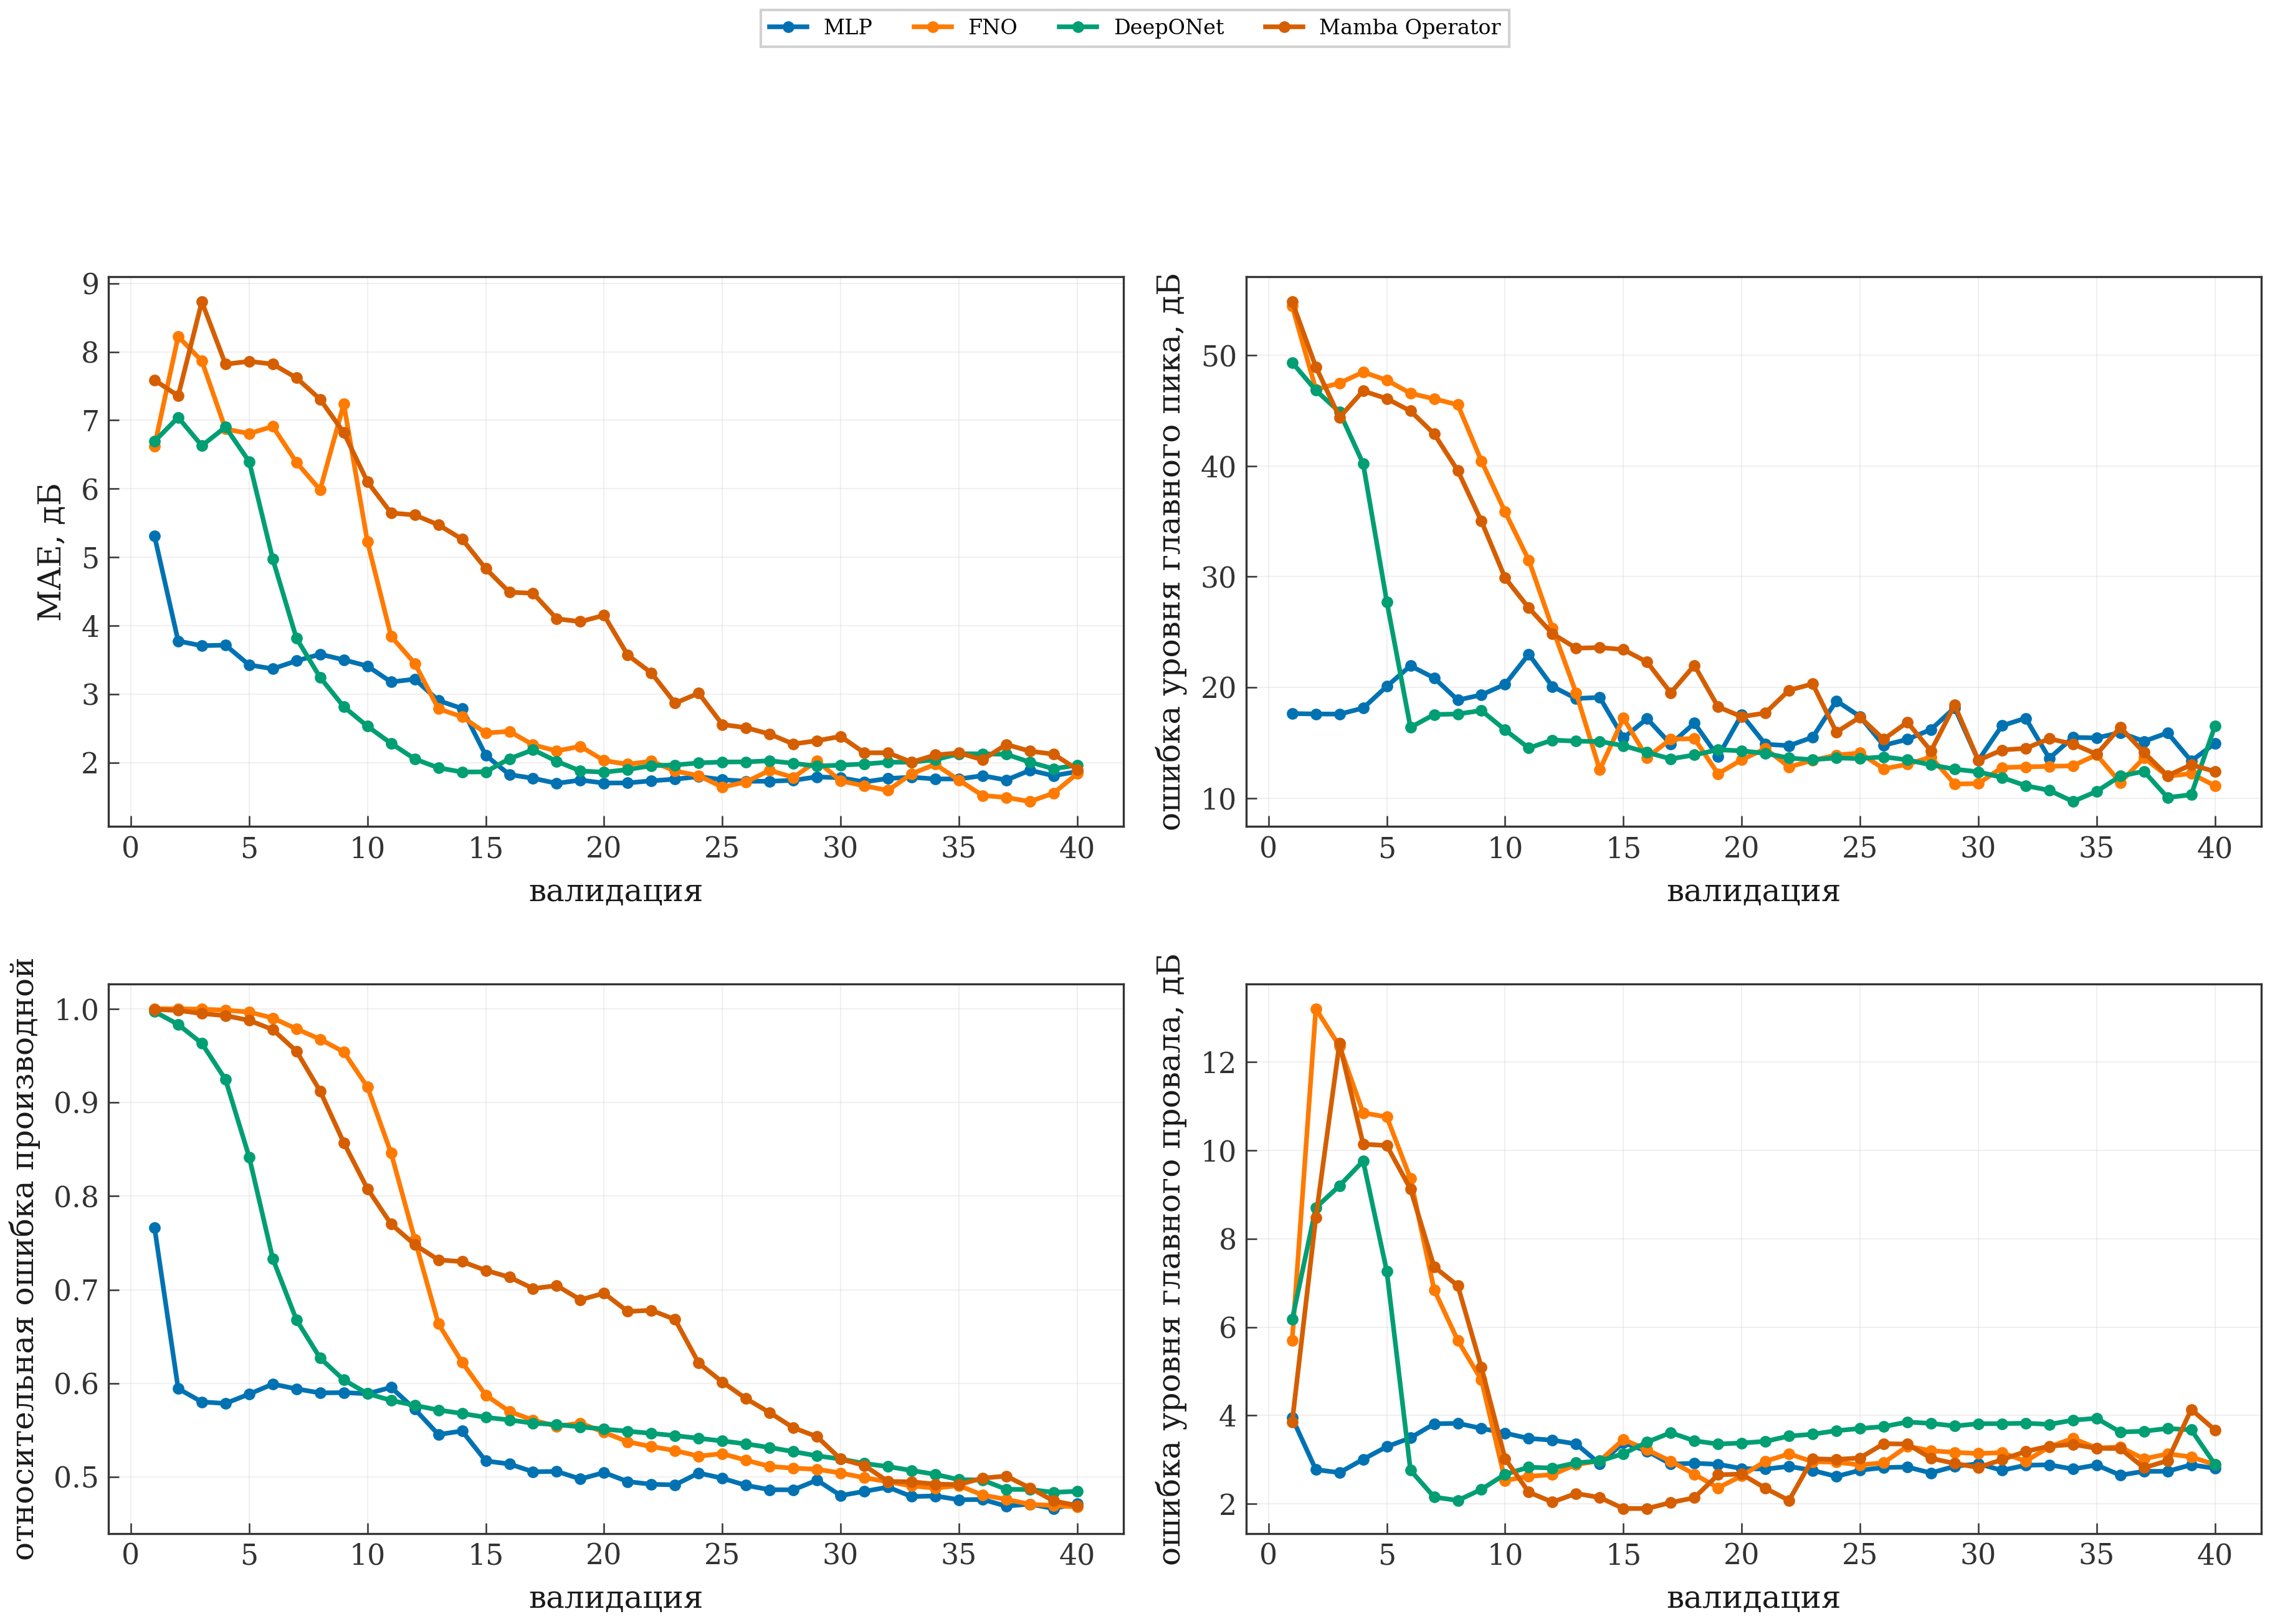
\includegraphics[width=0.95\textwidth]{images/метрики_mlp_fno_deep_mamba.png}
    \caption{Сравнение изменения валидационного MAE в процессе обучения для базовых архитектур MLP, FNO, DeepONet и Mamba Operator.}
    \label{fig:metrics_curves_comparison}
\end{figure}

\section{Модификации архитектуры DeepONet}
\label{sec:deeponet_modifications}

Благодаря разделению на независимые ветви (для геометрического профиля) и ствол (для частотной координаты), базовая архитектура DeepONet обладает значительным потенциалом для структурных изменений и является наиболее интересной моделью для исследования различных модификаций. В данном разделе рассматриваются различные архитектурные улучшения, направленные на повышение качества аппроксимации передаточных функций за счет учета пространственной переменности каналов и высокочастотных компонент спектра.

\subsection{Описание модификаций}
\label{subsec:modifications_description}

Во всех рассматриваемых модификациях сохраняется базовая идея DeepONet~\cite{lu2021learning}: геометрический профиль обрабатывается ветвью, частотная координата --- стволом, а итоговый спектральный отклик формируется на этапе слияния их латентных представлений. При этом в нашей работе изменения вносятся в один из трех узлов архитектуры:
\begin{itemize}
    \item \textbf{ветвь (branch)} --- когда требуется лучше учитывать локальные особенности профиля канала;
    \item \textbf{ствол (trunk)} --- когда требуется более гибко кодировать частотную зависимость;
    \item \textbf{блок слияния (fusion)} --- когда требуется заменить простое скалярное произведение на более выразительный механизм взаимодействия геометрии и частоты.
\end{itemize}

Таким образом, другие архитектуры встраиваются в DeepONet не как самостоятельные модели, а как замена или надстройка над одной из его стандартных подсетей. Были исследованы следующие варианты модификаций базовой модели:

\begin{enumerate}
    \item \textbf{Деформируемая ветвь (Deformable DeepONet)}~\cite{dai2017deformable}
    
    В этой конфигурации стандартные одномерные сверточные блоки ветви заменяются на деформируемые сверточные слои типа Deformable Convolutional Networks. Дополнительная сеть смещений вычисляет положения выборок для свертки по самому входному профилю, поэтому рецептивное поле ветви может локально смещаться к участкам резких сужений, расширений и неоднородностей. В контексте нашей задачи это означает, что модификация применяется именно к \emph{геометрическому энкодеру} DeepONet, тогда как ствол и правило слияния остаются базовыми.
    
    \item \textbf{Динамическая ветвь (Dynamic DeepONet)}~\cite{chen2020dynamic}
    
    Здесь в ветви используются слои динамической свертки: вместо одного фиксированного ядра каждый блок формирует взвешенную комбинацию из $K=4$ экспертных ядер, а веса смеси задаются небольшой routing-сетью по текущему входному профилю. Такая схема позволяет ветви адаптировать фильтрацию под различные типы геометрий. Иными словами, в нашей реализации идеи Dynamic Convolution модифицируют \emph{только branch-net}, не затрагивая trunk-net и финальный декодер.
    
    \item \textbf{Синусоидальный ствол (SIREN DeepONet)}~\cite{sitzmann2020siren}
    
    В этой модификации стандартный MLP ствола с активацией GELU заменяется на синусоидальную сеть SIREN с активацией $\sin(\omega_0 x)$ и параметром $\omega_0 = 10.0$. В реализации используется специализированная инициализация SIREN: для первого слоя веса выбираются из равномерного распределения на интервале $[-1/\text{in}, 1/\text{in}]$, а для скрытых слоев масштабируются как $\sqrt{6/\text{in}}/\omega_0$. Тем самым синусоидальная архитектура используется у нас как \emph{замена trunk-net}, отвечающего за представление частотной координаты. Несмотря на потенциальную выразительность, как показано в подразделе~\ref{subsec:modifications_comparison}, в текущей задаче такая конфигурация оказалась менее устойчивой к обучению.
    
    \item \textbf{Модуляция признаков FiLM (FiLM DeepONet)}~\cite{perez2018film}
    
    Механизм Feature-wise Linear Modulation используется нами для условной модуляции ствола признаками ветви. Латентный вектор геометрии с выхода branch-net преобразуется в параметры $\gamma$ и $\beta$, которые на каждом слое trunk-net выполняют аффинное преобразование промежуточных признаков. Таким образом, FiLM встраивается в DeepONet как \emph{межсетевая связь branch $\rightarrow$ trunk}, позволяющая частотному представлению зависеть от геометрии не только в финальном скалярном произведении, но и на промежуточных уровнях.
    
    \item \textbf{Билинейное слияние (Bilinear Fusion DeepONet)}~\cite{kim2016hadamard}
    
    В этой конфигурации классическое скалярное произведение между выходами ветви и ствола заменяется на более выразительное билинейное взаимодействие с рангом сжатия $128$. Геометрический и частотный латентные векторы сначала проецируются в общее пространство, после чего между ними вычисляется билинейная комбинация, способная моделировать нелинейные попарные зависимости. Следовательно, билинейная архитектура применяется у нас не к branch или trunk по отдельности, а именно к \emph{fusion-блоку} DeepONet.
    
    \item \textbf{Слияние через механизм внимания (Attention Fusion DeepONet)}~\cite{vaswani2017attention}
    Использует облегченный механизм перекрестного внимания (Cross-Attention) с размерностью внимания $d_{\mathrm{att}} = 64$ и $M = 8$ токенами памяти геометрии. Базисные векторы ствола $\mathbf{t}(f) \in \mathbb{R}^p$ ($p=128$) проецируются в запросы $\mathbf{q}(f) \in \mathbb{R}^{d_{\mathrm{att}}}$, а коэффициенты ветви $\mathbf{b} \in \mathbb{R}^p$ отображаются в набор токенов памяти для ключей $\mathbf{k} \in \mathbb{R}^{M \times d_{\mathrm{att}}}$ и значений $\mathbf{v} \in \mathbb{R}^{M \times d_{\mathrm{att}}}$ с помощью полносвязных слоев:
    \begin{align}
        \mathbf{q}(f) &= \mathbf{W}_q \operatorname{LayerNorm}(\mathbf{t}(f)) + \mathbf{b}_q, \\
        [\mathbf{k}; \mathbf{v}] &= \mathbf{W}_m \operatorname{LayerNorm}(\mathbf{b}) + \mathbf{b}_m.
    \end{align}
    Матрица внимания вычисляется как скалярное произведение запросов и ключей:
    \begin{equation}
        A_m(f) = \operatorname{softmax}_m \left( \frac{\mathbf{q}(f) \mathbf{k}_m^T}{\sqrt{d_{\mathrm{att}}}} \right),
    \end{equation}
    а результирующий вектор внимания имеет вид:
    \begin{equation}
        \mathbf{o}(f) = \sum_{m=1}^M A_m(f) \mathbf{v}_m.
    \end{equation}
    Итоговое предсказание АЧХ $\widehat{H}_{\mathrm{dB}}(f)$ вычисляется выходной головкой с добавлением масштабированного скалярного произведения (residual dot connection):
    \begin{equation}
        \widehat{H}_{\mathrm{dB}}(f) = \operatorname{OutputHead}(\mathbf{o}(f)) + \frac{1}{\sqrt{p}} \sum_{j=1}^p b_j \cdot t_j(f) + b_{\mathrm{bias}}.
    \end{equation}
    В нашей постановке attention-механизм заменяет \emph{стандартный узел слияния} DeepONet: trunk формирует запрос, а branch --- компактную память геометрии. Это позволяет снизить вычислительную сложность внимания с квадратичной по частоте $O(N_f^2)$ до линейной $O(N_f \cdot M)$.
    
    \item \textbf{Слияние с Mamba (Mamba Fusion DeepONet)}~\cite{dao2024mamba2,gu2024mamba}
    
    Использует блоки Mamba/Mamba-2 на этапе слияния геометрического и частотного представлений. После кодирования branch-net и trunk-net их признаки объединяются в последовательность токенов, которая затем обрабатывается state-space блоком. В отличие от базового DeepONet, где взаимодействие ветви и ствола сводится к одному скалярному произведению, Mamba Fusion выполняет \emph{последовательностный fusion-декодер}, способный учитывать более сложные и дальнодействующие зависимости между профилем канала и частотным запросом.
\end{enumerate}

\subsection{Сравнение точности модификаций}
\label{subsec:modifications_comparison}

Сравнение качества аппроксимации переоцененных нейросетевых архитектур проводилось на одном и том же валидационном наборе данных. В таблице~\ref{tab:modifications_comparison} приведены четыре основные валидационные метрики качества для моделей после 40 эпох обучения. Для каждой модели указаны средние значения и стандартные отклонения, полученные по 10 независимым прогонам валидации.

\begin{table}[H]
    \centering
    \caption{Сравнение нейросетевых моделей и архитектурных модификаций после 40 эпох обучения; приведены средние значения и стандартные отклонения метрик по 10 независимым прогонам валидации}
    \label{tab:modifications_comparison}
    \resizebox{\textwidth}{!}{%
    \begin{tabular}{|l|c|c|c|c|}
        \hline
        Модель & MAE, дБ & Ошибка уровня пика, дБ & Ошибка произв. & Ошибка уровня провала, дБ \\
        \hline
        MLP & 1.6806 $\pm$ 0.0065 & 14.5609 $\pm$ 0.0715 & 0.4566 $\pm$ 0.0012 & 2.7936 $\pm$ 0.0068 \\
        MLP MSE baseline & 1.2166 $\pm$ 0.0024 & 13.8483 $\pm$ 0.0740 & 0.4910 $\pm$ 0.0014 & \textbf{1.8010 $\pm$ 0.0089} \\
        FNO & 1.4445 $\pm$ 0.0032 & 13.9382 $\pm$ 0.0977 & 0.4655 $\pm$ 0.0020 & 2.9951 $\pm$ 0.0093 \\
        DeepONet & 1.8705 $\pm$ 0.0038 & \textbf{10.4937 $\pm$ 0.0979} & 0.4730 $\pm$ 0.0019 & 3.7042 $\pm$ 0.0117 \\
        Mamba Operator & 1.7041 $\pm$ 0.0054 & 16.1968 $\pm$ 0.0676 & 0.4615 $\pm$ 0.0011 & 3.3763 $\pm$ 0.0074 \\
        \hline
        FiLM DeepONet & 2.1063 $\pm$ 0.0020 & 13.9952 $\pm$ 0.0908 & 0.4863 $\pm$ 0.0017 & 3.4917 $\pm$ 0.0071 \\
        Bilinear Fusion DeepONet & 1.8596 $\pm$ 0.0037 & 10.9087 $\pm$ 0.1017 & 0.4271 $\pm$ 0.0021 & 3.7707 $\pm$ 0.0083 \\
        SIREN DeepONet & 3.7186 $\pm$ 0.0009 & 28.7148 $\pm$ 0.0621 & 0.8830 $\pm$ 0.0002 & 2.1131 $\pm$ 0.0117 \\
        Dynamic DeepONet & 2.1426 $\pm$ 0.0063 & 13.2626 $\pm$ 0.0666 & 0.4941 $\pm$ 0.0016 & 4.2483 $\pm$ 0.0103 \\
        Deformable DeepONet & 2.0274 $\pm$ 0.0050 & 11.0803 $\pm$ 0.0886 & 0.4794 $\pm$ 0.0019 & 4.2219 $\pm$ 0.0098 \\
        \textbf{Mamba Fusion DeepONet} & \textbf{1.0016 $\pm$ 0.0031} & 9.6045 $\pm$ 0.1124 & \textbf{0.3311 $\pm$ 0.0015} & 2.7235 $\pm$ 0.0074 \\
        \hline
    \end{tabular}%
    }
\end{table}

Как видно из результатов сравнения, среди базовых архитектур модель \textbf{MLP MSE baseline} демонстрирует наименьшие значения глобальной ошибки MAE ($1.2166 \pm 0.0024$ дБ) и ошибки уровня главного провала ($1.8010 \pm 0.0089$ дБ), однако уступает другим подходам по ошибке производной спектра ($0.4910 \pm 0.0014$). Среди базовых архитектур \textbf{DeepONet} точнее передает уровень доминирующего резонансного пика ($10.4937 \pm 0.0979$ дБ), а \textbf{FNO} обеспечивает более низкую глобальную ошибку, чем базовый DeepONet и Mamba Operator.

Среди всех исследованных модификаций архитектура \textbf{Mamba Fusion DeepONet} демонстрирует наилучшую общую точность: средняя абсолютная ошибка MAE снижается до $1.0016 \pm 0.0031$ дБ, что соответствует улучшению примерно на $46.5\%$ относительно базового DeepONet, а относительная ошибка по производной составляет всего $0.3311 \pm 0.0015$. По ошибке уровня главного резонансного пика наилучший результат также показывает \textbf{Mamba Fusion DeepONet} ($9.6045 \pm 0.1124$ дБ). При этом синусоидальный ствол \textbf{SIREN DeepONet}, как и прежде, демонстрирует заметно худшие значения глобальных спектральных метрик (MAE $3.7186 \pm 0.0009$ дБ и ошибка уровня пика $28.7148 \pm 0.0621$ дБ), несмотря на сравнительно низкую ошибку уровня главного провала.

Сравнение кривых сходимости функций потерь и валидационных метрик в процессе обучения для модификаций представлено на рис.~\ref{fig:loss_modifications} и рис.~\ref{fig:metrics_modifications}. Предсказанные АЧХ на тестовом образце для всех исследованных моделей приведены на рис.~\ref{fig:all_spectrums}.

\begin{figure}[H]
    \centering
    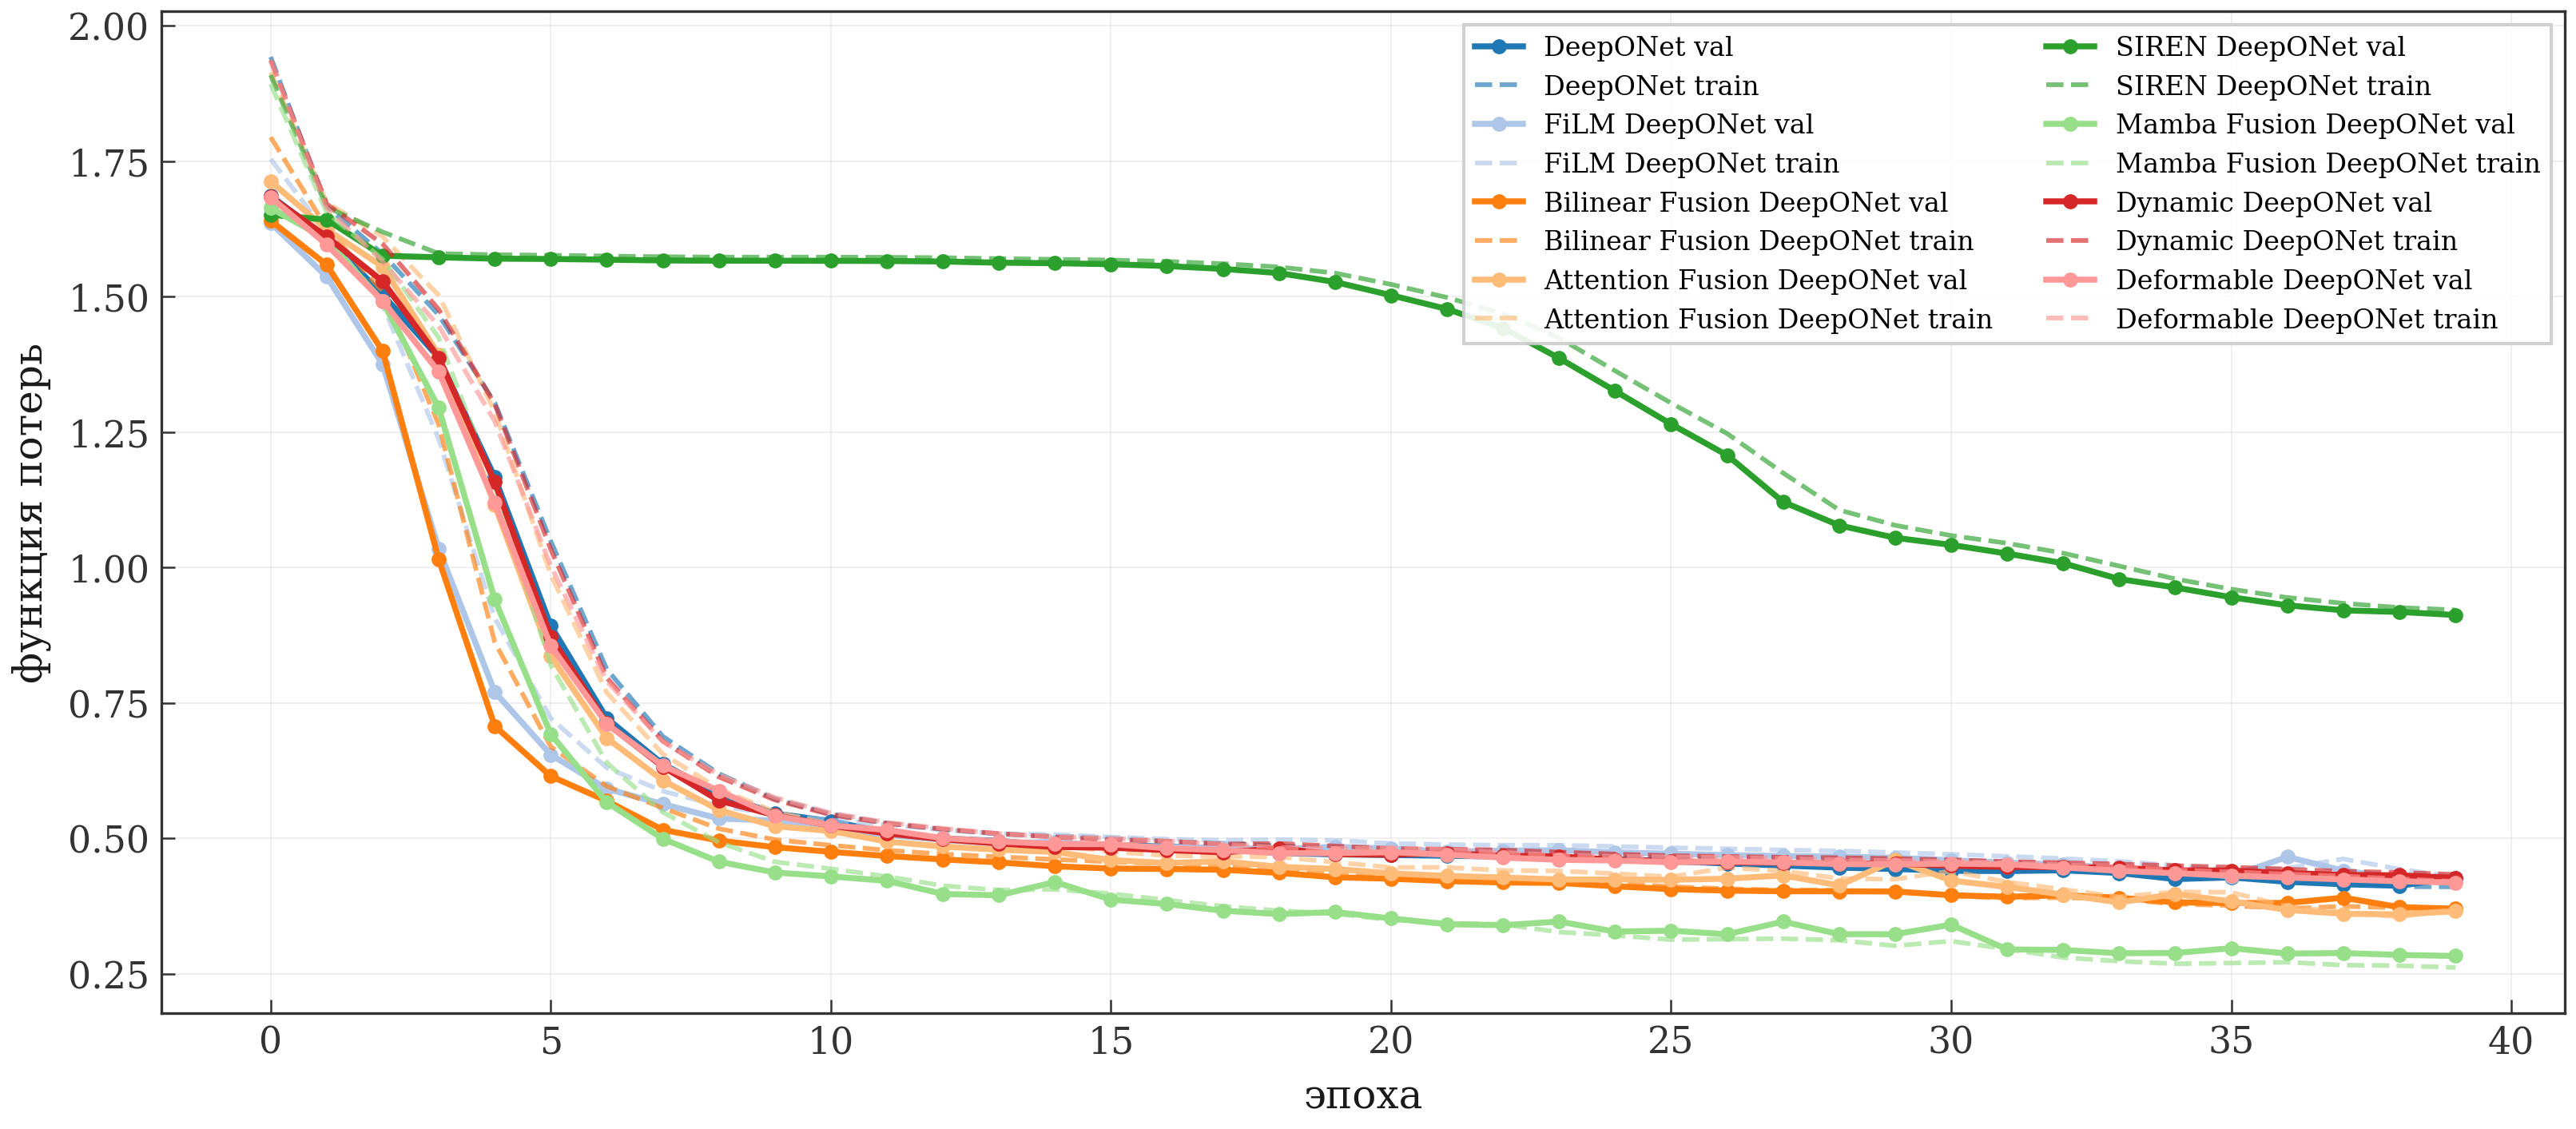
\includegraphics[width=0.95\textwidth]{images/функции_потерь_модификаций_deeponet.png}
    \caption{Сходимость комбинированного лосса $L_{\text{total}}$ для модификаций DeepONet.}
    \label{fig:loss_modifications}
\end{figure}

\begin{figure}[H]
    \centering
    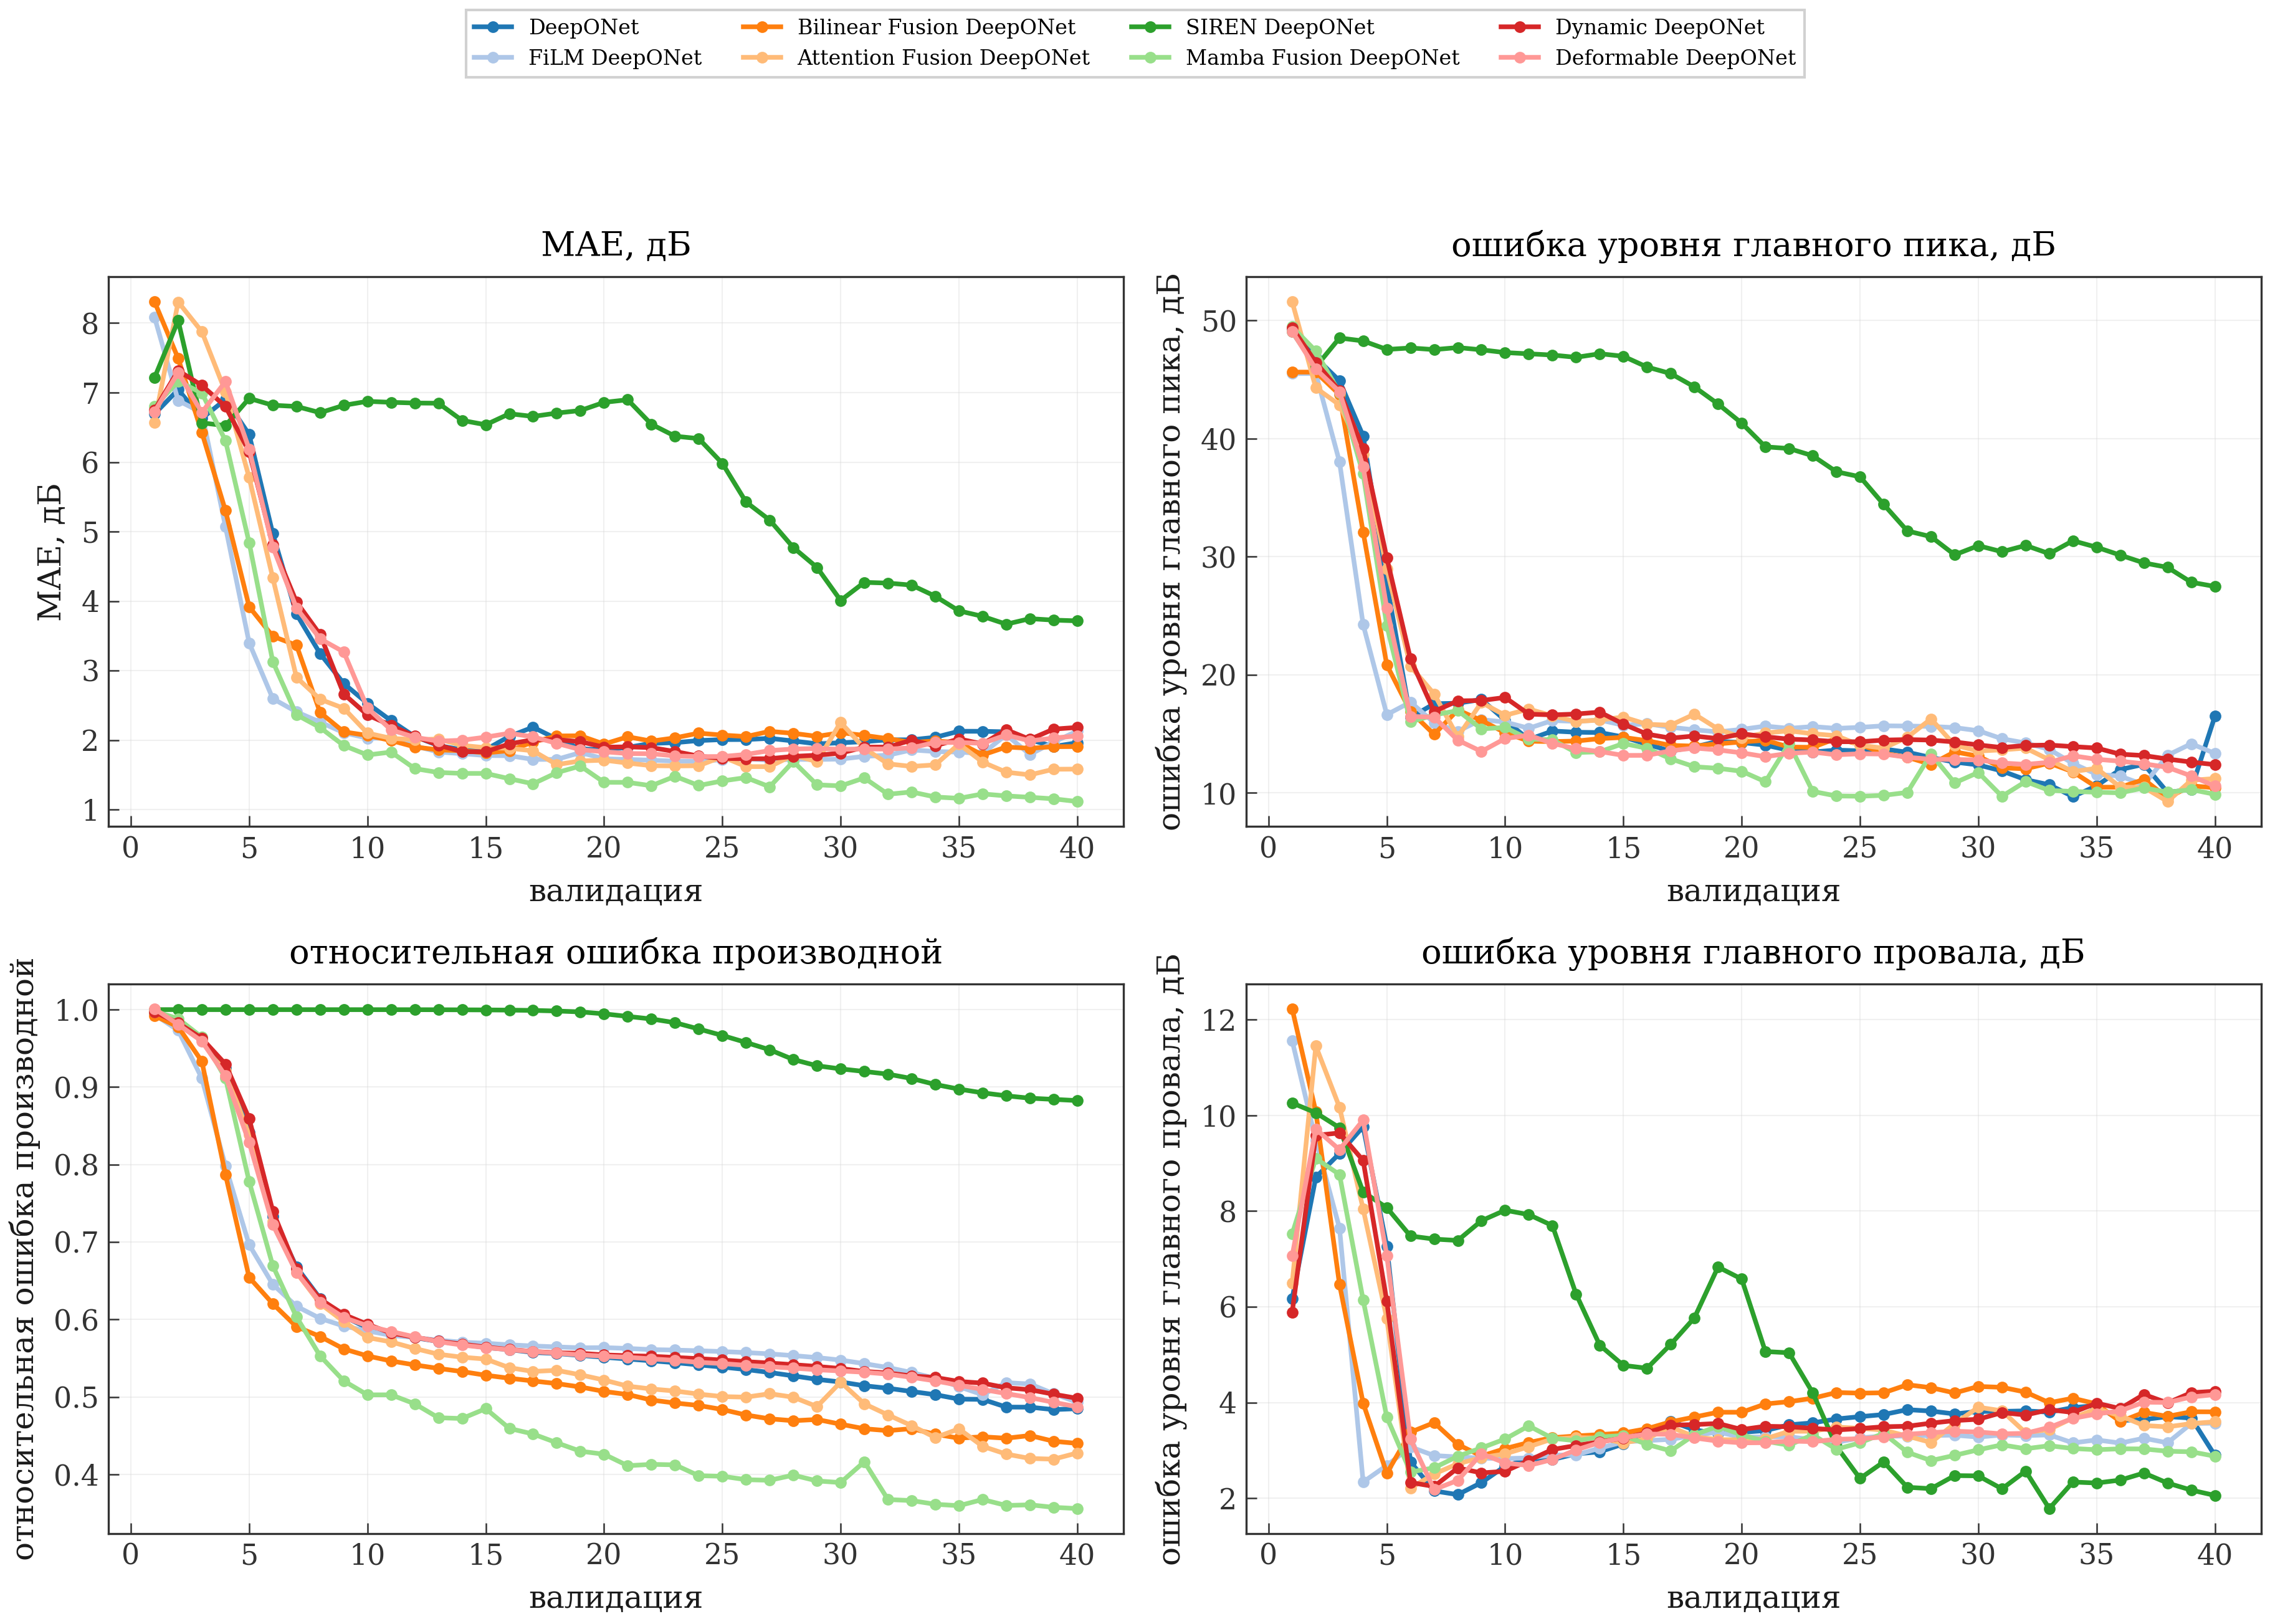
\includegraphics[width=0.95\textwidth]{images/метрики_модификаций_deeponet.png}
    \caption{Сравнение изменения валидационного MAE в процессе обучения для модификаций DeepONet.}
    \label{fig:metrics_modifications}
\end{figure}

\begin{figure}[H]
    \centering
    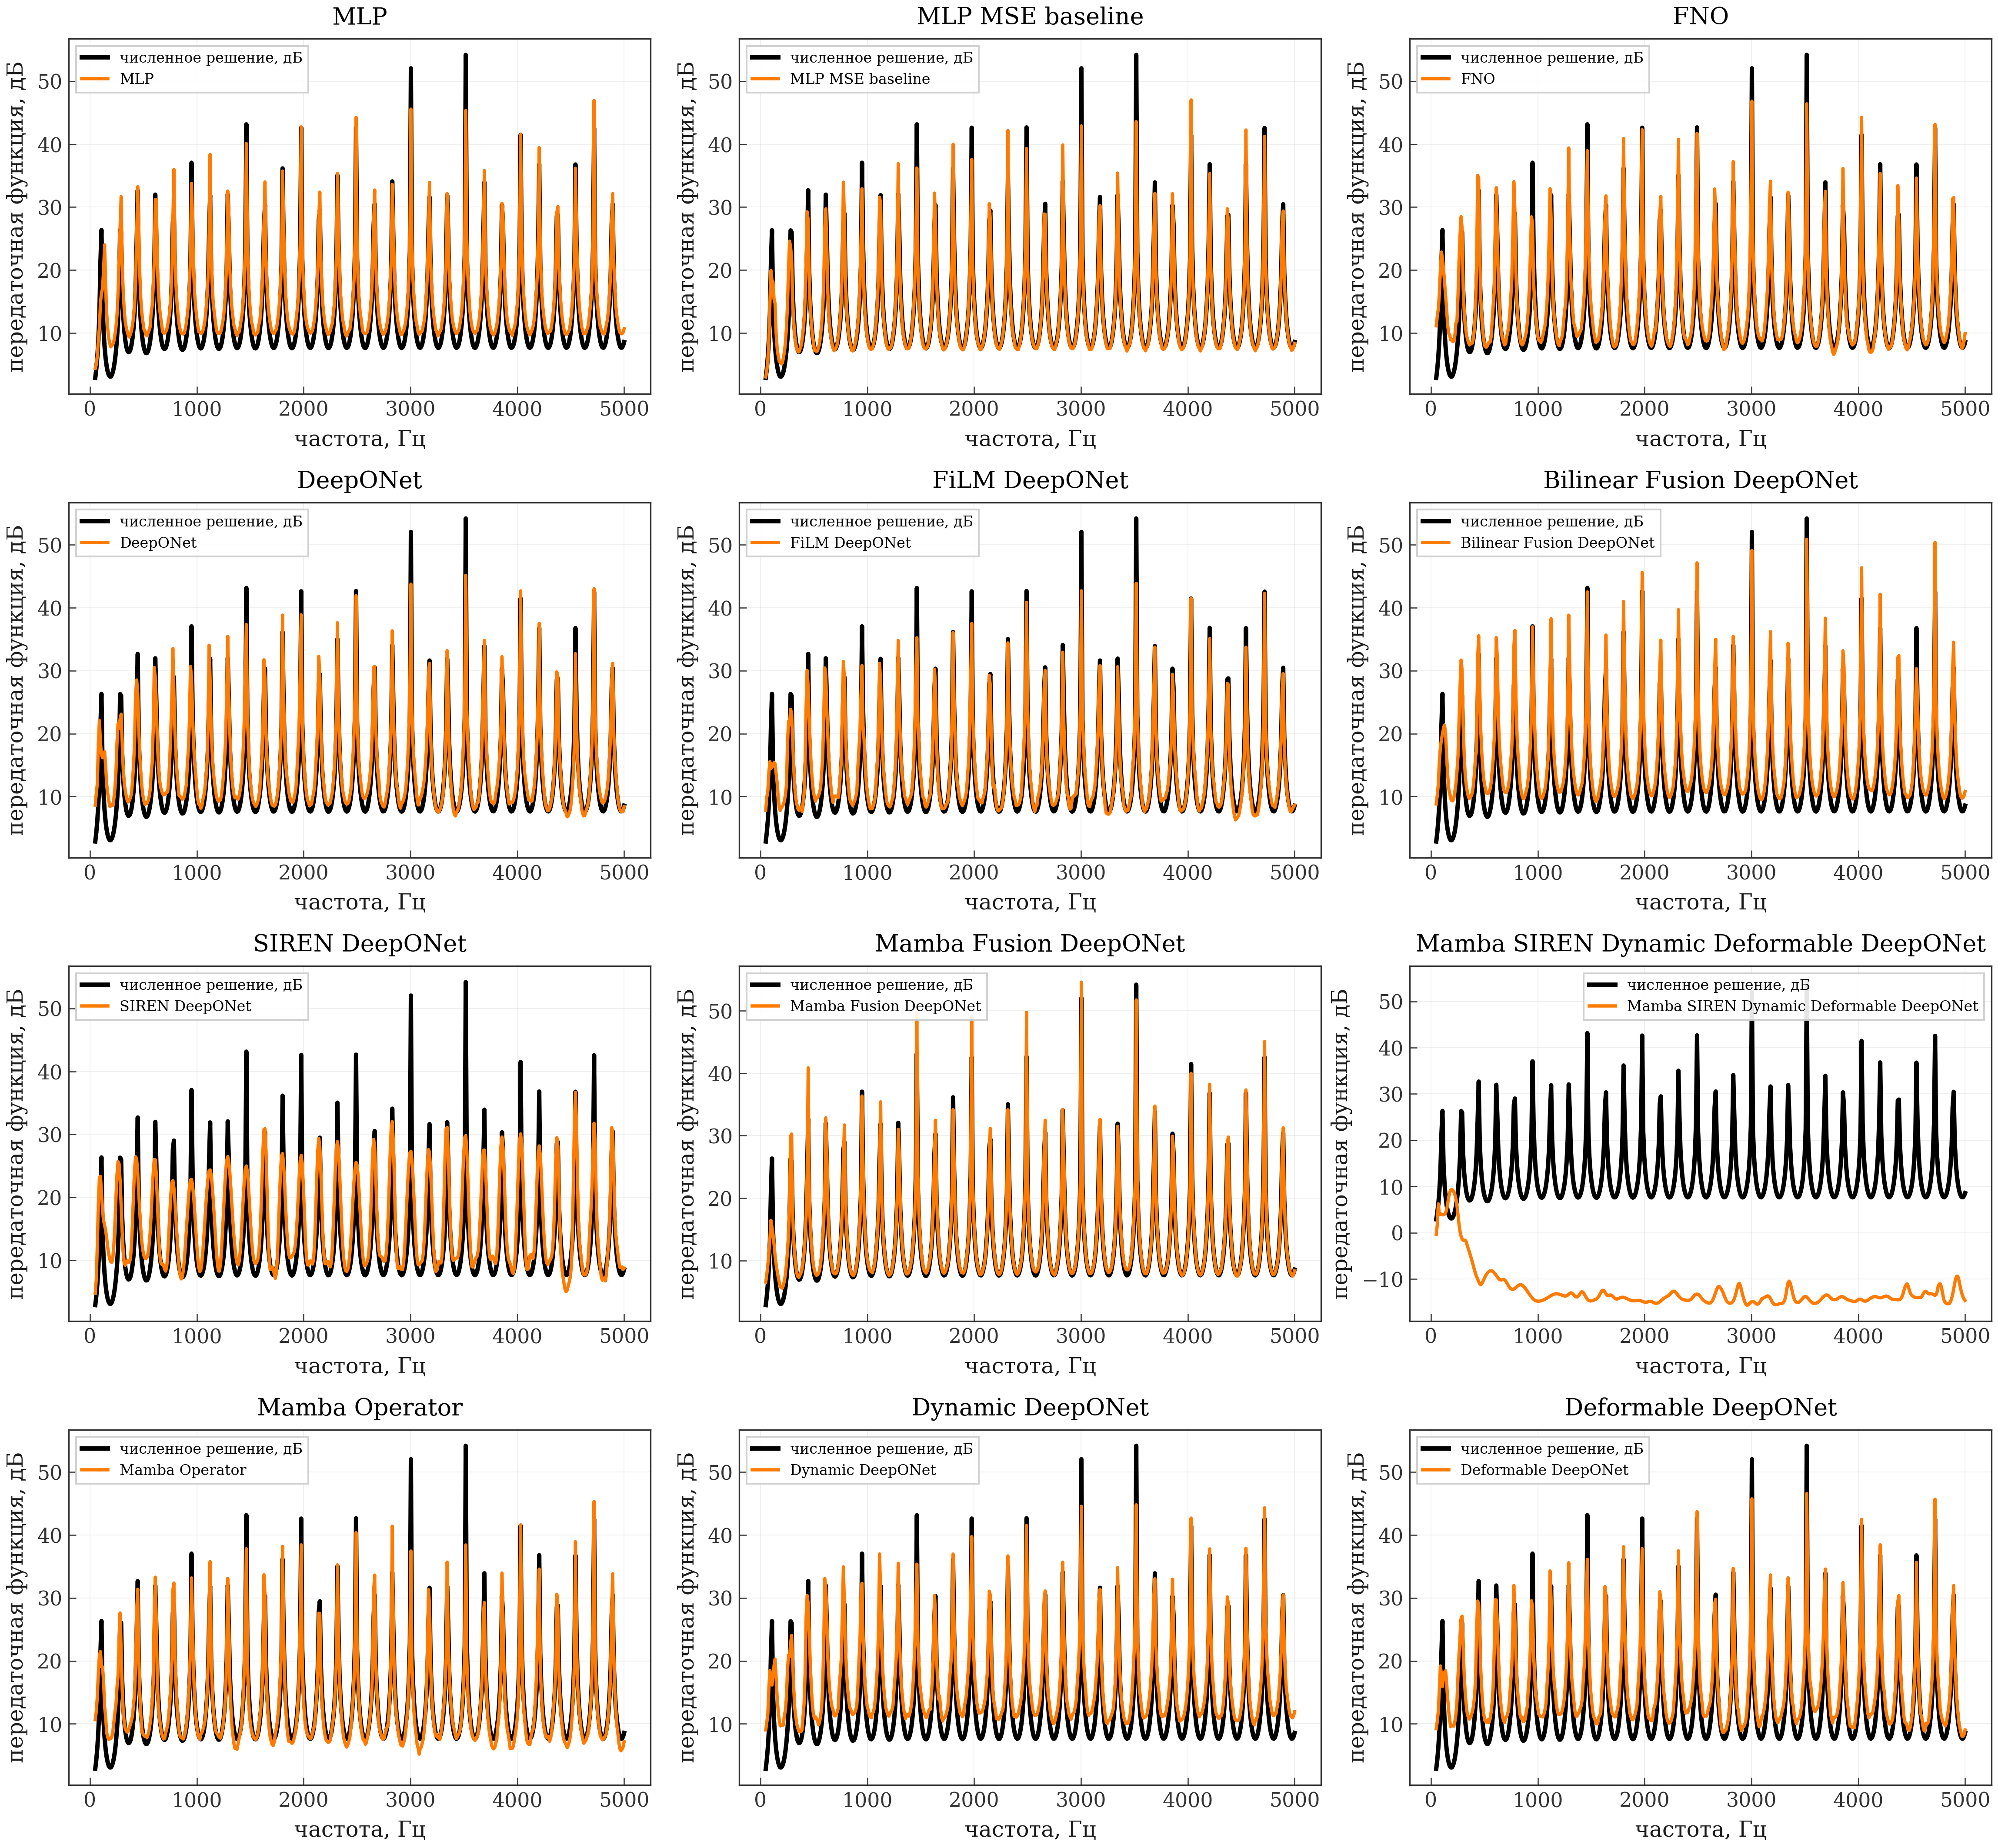
\includegraphics[width=0.95\textwidth]{images/all.png}
    \caption{Сравнение эталонной АЧХ, полученной опорным численным решателем, и предсказаний всех исследованных нейросетевых моделей для тестового резонатора.}
    \label{fig:all_spectrums}
\end{figure}

\subsection{Сравнение моделей при длительном обучении}
\label{subsec:mamba_70_comparison}

Для исследования предельной сходимости и потенциала оптимизации моделей, основанных на механизмах пространства состояний (Mamba), был проведен дополнительный эксперимент с увеличением длительности обучения до 70 эпох. В данном эксперименте оценивались три конфигурации: базовый оператор \texttt{Mamba Operator}, модификация \texttt{Mamba Fusion DeepONet} и наиболее сложная гибридная архитектура \texttt{Mamba SIREN Dynamic Deformable DeepONet}, сочетающая Mamba-блоки с синусоидальным стволом SIREN, а также деформируемыми и динамическими свертками в ветви. При этом для двух архитектур на основе DeepONet использовался размер батча 32, тогда как для \texttt{Mamba Operator} размер батча был уменьшен до 4 из-за более высоких затрат видеопамяти.

Результаты сравнения лучших значений метрик на валидационной выборке приведены в таблице~\ref{tab:mamba_70_comparison}.

\begin{table}[H]
    \centering
    \caption{Сравнение нейросетевых моделей на основе Mamba при длительном обучении (70 эпох); приведены средние значения метрик по 10 независимым прогонам валидации}
    \label{tab:mamba_70_comparison}
    \label{tab_count} % Для подсчета таблиц в аннотации
    \resizebox{\textwidth}{!}{%
    \begin{tabular}{|l|c|c|c|c|}
        \hline
        Модель & MAE, дБ & Ошибка уровня пика, дБ & Ошибка произв. & Ошибка уровня провала, дБ \\
        \hline
        Mamba Operator & 1.7041 & 16.1968 & 0.4615 & 3.3763 \\
        Mamba Fusion DeepONet & 1.0016 & 9.6045 & 0.3311 & 2.7235 \\
        \textbf{Mamba SIREN Dynamic Deformable DeepONet} & \textbf{0.9115} & \textbf{9.5806} & \textbf{0.3140} & \textbf{1.7679} \\
        \hline
    \end{tabular}%
    }
\end{table}

Анализ усредненных по 10 независимым прогонам результатов показывает, что гибридная архитектура \textbf{Mamba SIREN Dynamic Deformable DeepONet} превосходит остальные конфигурации по всем показателям. Она достигает наименьшей средней абсолютной ошибки MAE $= 0.9115$ дБ (улучшение примерно на $9\%$ по сравнению с Mamba Fusion DeepONet и на $46.5\%$ по сравнению с Mamba Operator). Также данная модель демонстрирует наименьшую ошибку передачи уровня доминирующего резонансного пика ($9.5806$ дБ), производной спектра ($0.3140$) и наиболее точное определение уровня главного провала ($1.7679$ дБ).

Это подтверждает гипотезу о том, что интеграция блоков пространства состояний Mamba-2 для моделирования пространственной связности в сочетании с синусоидальным стволом (SIREN) для высокочастотного спектрального разрешения и адаптивными пространственными свертками дает выраженный синергетический эффект при длительном обучении.

Кривые изменения функций потерь $L_{\text{total}}$ и валидационного MAE в процессе 70 эпох обучения представлены на рис.~\ref{fig:loss_mamba_70} и рис.~\ref{fig:metrics_mamba_70}.

\begin{figure}[H]
    \centering
    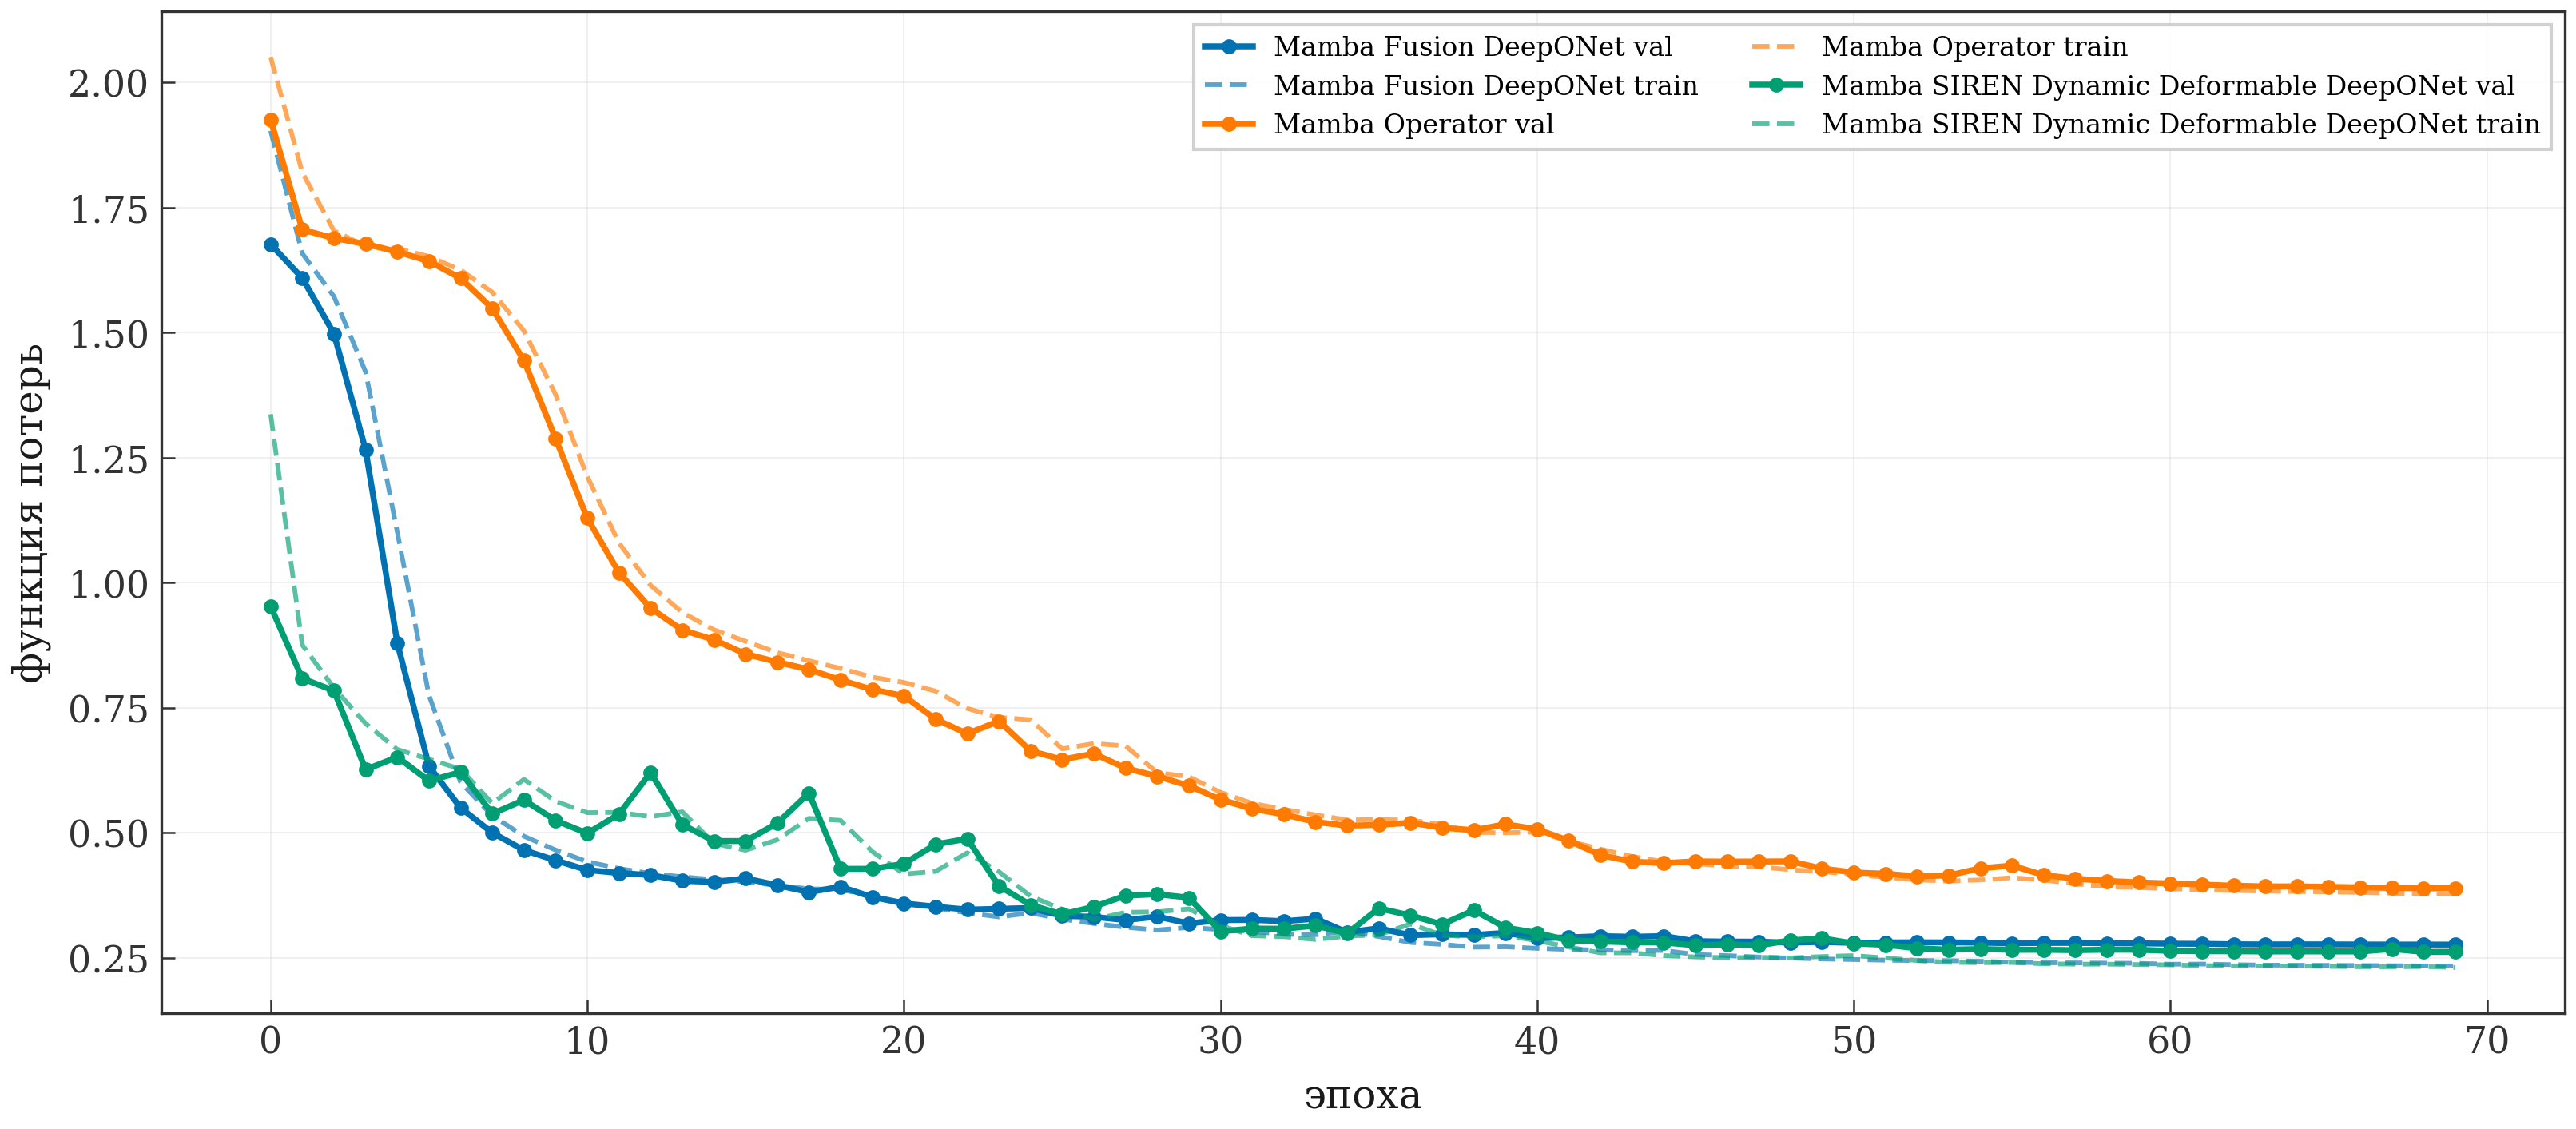
\includegraphics[width=0.95\textwidth]{images/функции_потерь_mamba_70.png}
    \caption{Сходимость комбинированного лосса $L_{\text{total}}$ при длительном обучении (70 эпох) для моделей на основе Mamba.}
    \label{fig:loss_mamba_70}
\end{figure}

\begin{figure}[H]
    \centering
    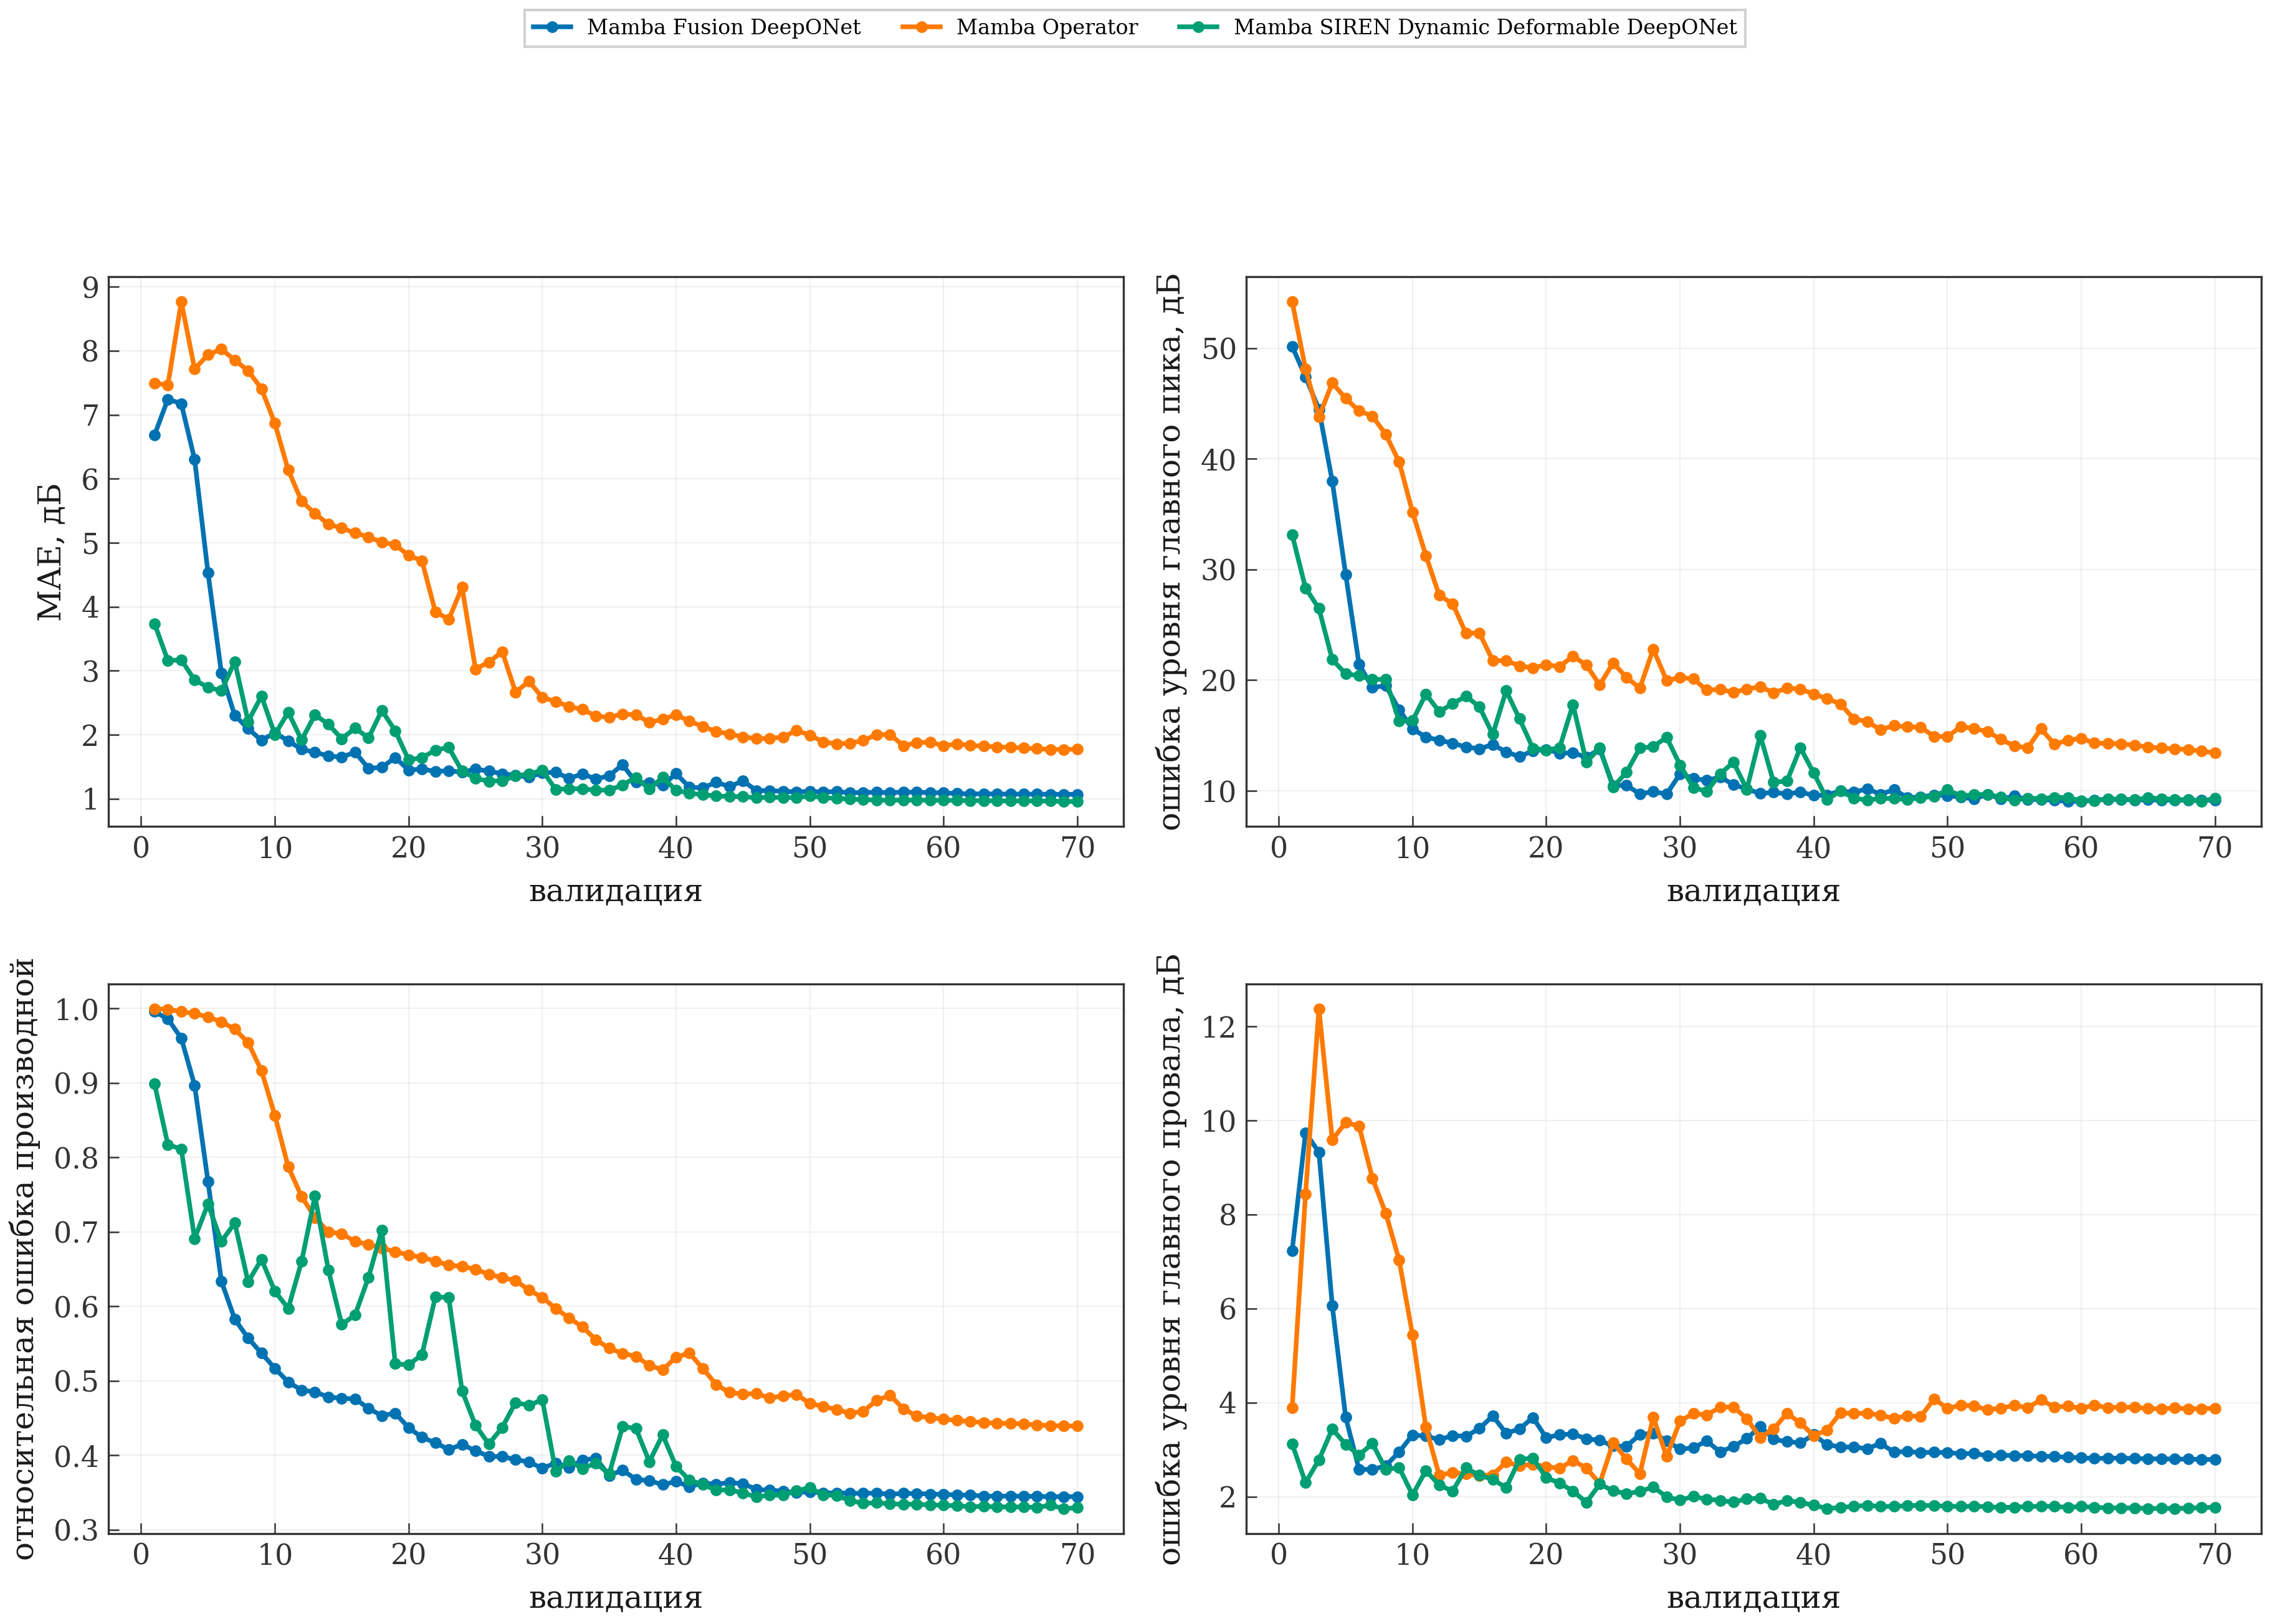
\includegraphics[width=0.95\textwidth]{images/метрики_mamba_70.png}
    \caption{Сравнение изменения валидационного MAE при длительном обучении (70 эпох) для моделей на основе Mamba.}
    \label{fig:metrics_mamba_70}
\end{figure}

\section{Сравнение скорости работы нейросетей и численных решателей}
\label{sec:speed_comparison}

Важным преимуществом нейросетевых суррогатных моделей является высокая скорость работы. Дополнительно исследовалась зависимость времени вычисления от плотности дискретизации сетки частот и разбиения геометрии. На рис.~\ref{fig:runtime_frequency_discretization} показано, как время работы конического решателя масштабируется по сетке частотных точек $N_f$ и пространственных сегментов $N_s$.

\begin{figure}[H]
    \centering
    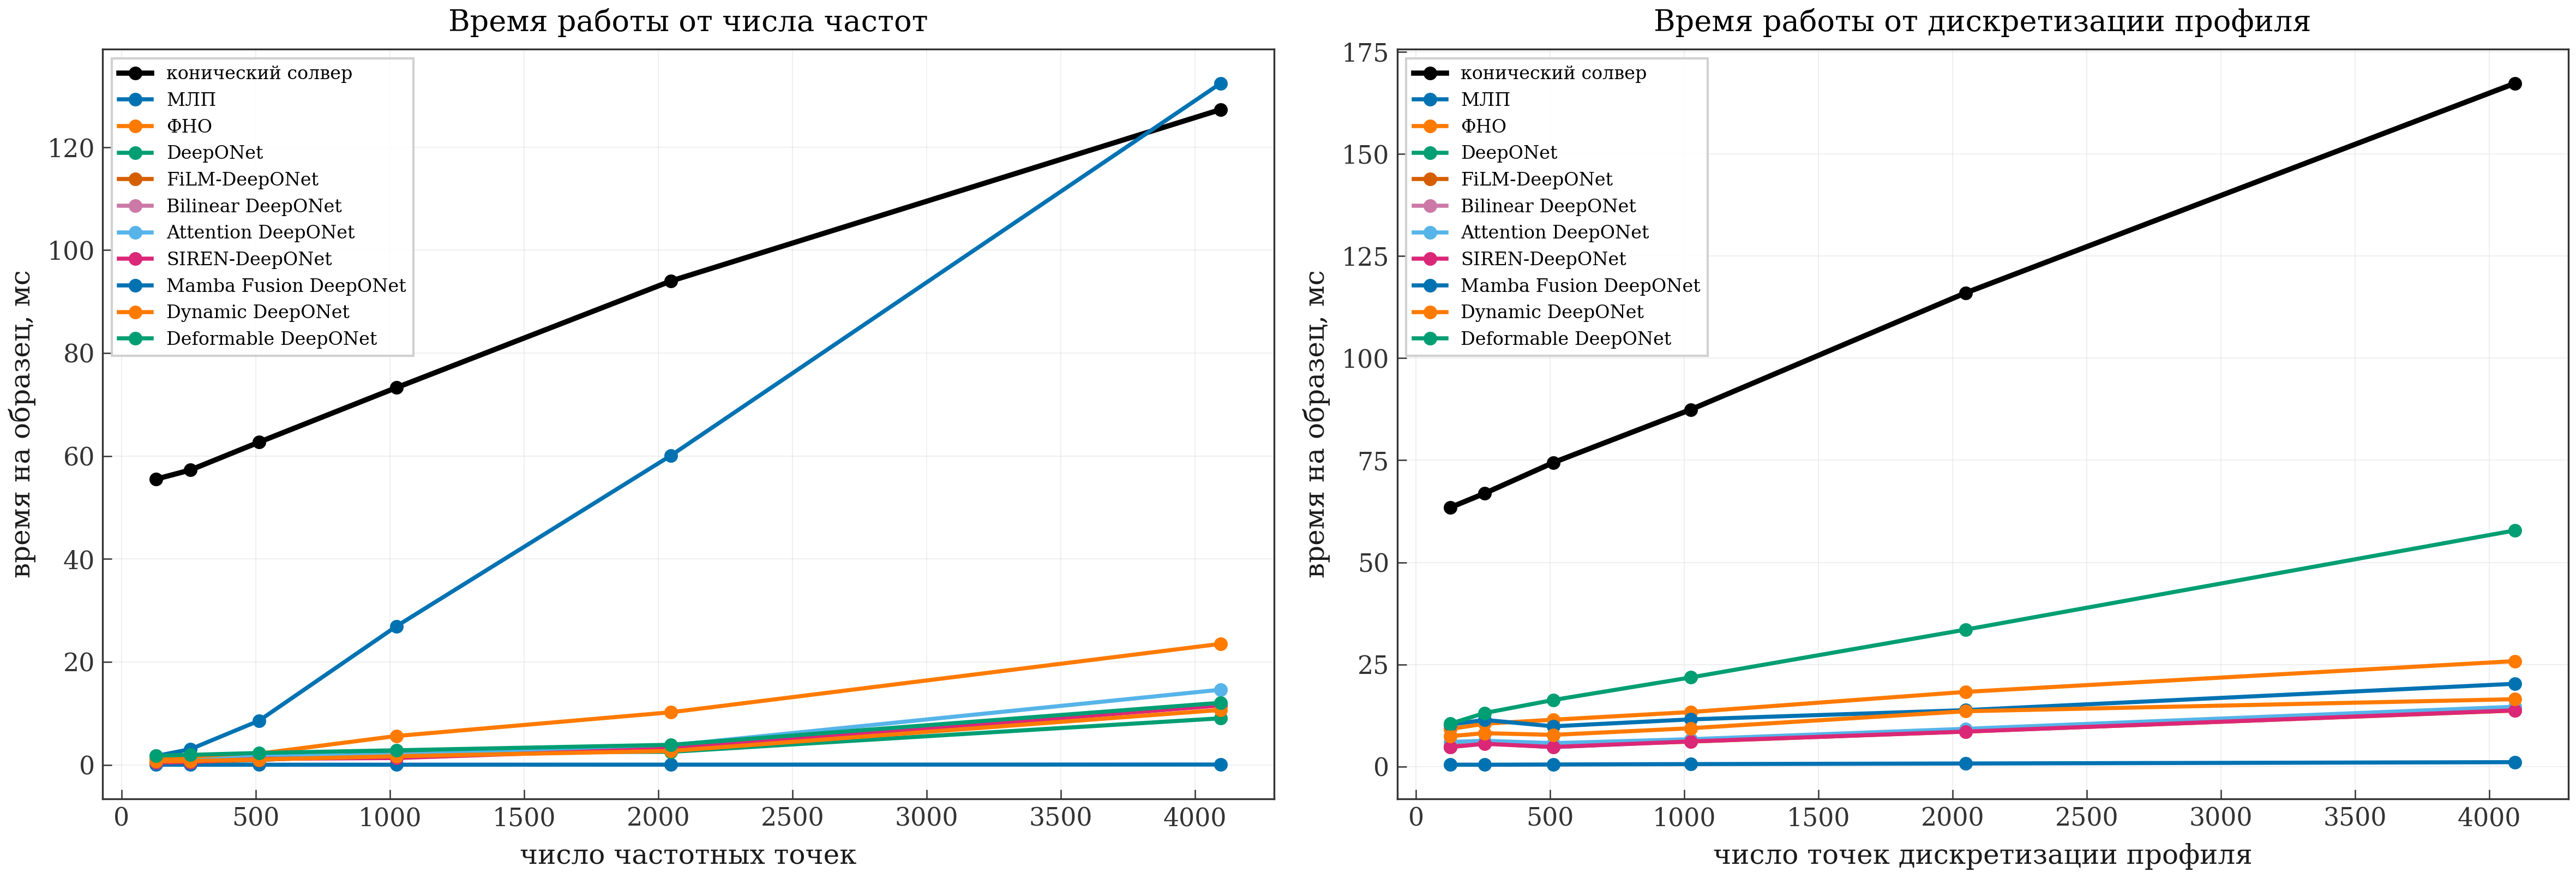
\includegraphics[width=0.95\textwidth]{images/время_работы_от_числа_частот_и_дискретизации.png}
    \caption{Время прямого расчета в зависимости от размера частотной сетки и дискретизации профиля.}
    \label{fig:runtime_frequency_discretization}
\end{figure}

Для численных решателей время вычислений возрастает примерно линейно от $N_s$ и $N_f$, так как алгоритм требует последовательного перемножения $N_s$ матриц передачи размерности $2 \times 2$ для каждой из $N_f$ частот, что дает сложность $O(N_s \cdot N_f)$. В отличие от численных подходов, нейросети выполняют вычисления параллельно с использованием оптимизированных библиотек линейной алгебры. Их время инференса в исследуемом диапазоне разрешений растет значительно слабее и хорошо маскируется батчевой и аппаратной параллельностью, обеспечивая ускорение работы на несколько порядков на высоких разрешениях сетки.

Следует отметить, что для сверхмалых сеток ($N_s < 10, N_f < 100$) компилируемый C++ TMM-решатель может работать быстрее из-за накладных расходов фреймворка PyTorch на инициализацию вычислений. Однако в практическом диапазоне размерностей суррогатные нейросетевые модели значительно превосходят классические методы по быстродействию.

\chapter{Результаты численного моделирования и сравнительный анализ}
\label{ch:results}

В данной главе представлены результаты анализа точности цилиндрической и конической аппроксимаций волновода, сравнение производительности реализованных численных решателей, а также результаты применения нейросетевых моделей для решения прямой и обратной задач волноводной акустики.

\section{Сравнение точности цилиндрической и конической аппроксимаций}
\label{sec:comparison_approx}

Для гладких геометрий (например, экспоненциального или катеноидального рупора) профиль площади поперечного сечения аппроксимируется набором дискретных элементов. Было проведено исследование сходимости решения при увеличении числа сегментов $N$ для цилиндрической и конической аппроксимаций.

В таблице~\ref{tab:errors} приведены значения среднеквадратичной ошибки (RMSE) для первых трех резонансных частот в зависимости от числа сегментов разбиения.

\begin{table}[h!]
    \centering
    \caption{Сравнение среднеквадратичной ошибки (RMSE, Гц) резонансных частот}
    \label{tab:errors}
    \begin{tabular}{|c|c|c|c|c|}
        \hline
        \multirow{2}{*}{Число сегментов $N$} & \multicolumn{2}{c|}{Цилиндрическая TMM} & \multicolumn{2}{c|}{Коническая TMM} \\
        \cline{2-5}
        & Резонанс 1 & Резонанс 2 & Резонанс 1 & Резонанс 2 \\
        \hline
        10  & 15.4 & 45.2 & 2.1  & 5.8  \\
        20  & 7.8  & 22.1 & 0.5  & 1.4  \\
        50  & 3.1  & 8.9  & 0.08 & 0.22 \\
        100 & 1.5  & 4.4  & 0.02 & 0.05 \\
        \hline
    \end{tabular}
\end{table}

Данные таблицы показывают, что коническая аппроксимация обеспечивает сходимость примерно на порядок быстрее по сравнению с цилиндрической при одинаковом числе сегментов $N$. Это объясняется более точным представлением производной площади $dA/dx$ в узлах сетки.

\section{Сравнение производительности решателей}
\label{sec:performance}

Проведено сравнение времени выполнения расчетов (в секундах) на стандартном наборе тестовых геометрий для Python-версии FDTD и C++ версии TLM. Результаты приведены в таблице~\ref{tab:performance}.

\begin{table}[h!]
    \centering
    \caption{Время выполнения расчета (в секундах) для 10000 временных шагов}
    \label{tab:performance}
    \begin{tabular}{|l|c|c|c|}
        \hline
        Метод & Язык реализации & Время работы (с) & Ускорение \\
        \hline
        FDTD (Webster) & Python & 2.45 & 1.0x \\
        TLM (Cylinder) & C++ & 0.08 & 30.6x \\
        \hline
    \end{tabular}
    \label{tab_count} % Для подсчета таблиц в аннотации
\end{table}

Использование C++ для реализации TLM-решателя позволило получить более чем 30-кратное ускорение расчетов во временной области, что критически важно для оптимизационных задач и обучения нейросетей на больших базах данных геометрий.

\section{Применение нейросетевого оператора (FNO)}
\label{sec:fno}

В качестве альтернативы традиционным численным решателям исследован подход на основе нейросетевого оператора Фурье (Fourier Neural Operator, FNO), обученного прогнозировать спектральный отклик (передаточную функцию $H_{\mathrm{dB}}(f)$) волновода по заданному дискретному профилю площадей сечений $\mathbf{a}$. 

В процессе валидации обученная модель FNO показала высокую точность аппроксимации: средняя абсолютная ошибка (MAE) по всему частотному диапазону составила $1.4299$ дБ, ошибка определения положения резонанса составила $11.1108$ дБ, а относительная ошибка по производной спектра --- $0.4680$ (подробные результаты приведены в табл.~\ref{tab:modifications_comparison} в главе~\ref{ch:direct_problem}). 

Благодаря параллельным тензорным вычислениям, время инференса FNO-модели на одном объекте составляет менее $1$ мс, что обеспечивает ускорение расчетов на несколько порядков по сравнению с классическими численными решателями на плотных сетках и делает данный подход перспективным для акустического моделирования в задачах реального времени.

\section{Решение обратной задачи восстановления геометрии}
\label{sec:inverse_problem}

Обратная задача волноводной акустики заключается в восстановлении продольного профиля площади поперечного сечения $A(x)$ волновода по заданной передаточной функции $H(f)$ (АЧХ). Данная задача является некорректно поставленной по Адамару из-за нелинейности отображения, а также физической неединственности решения (несколько существенно различающихся геометрий могут иметь крайне близкие спектральные отклики).

В рамках данной работы были исследованы два принципиально разных класса методов решения обратной задачи:
\begin{enumerate}
    \item Оптимизационные методы в пространстве параметров (градиентный спуск с обратным распространением ошибки через дифференцируемый нейросетевой эмулятор и стохастический поиск методом Метрополиса --- MCMC).
    \item Нейросетевой подход, основанный на обучении сверточной архитектуры типа UNet для прямого отображения спектральной карты в геометрический профиль.
\end{enumerate}

\subsection{Оптимизационные методы: градиентный спуск и метод Метрополиса}
\label{subsec:opt_methods}

В первом подходе обратная задача формулируется как минимизация невязки между целевой АЧХ $H_{\mathrm{target}}(f)$ и откликом текущей геометрии $\mathcal{F}_{\theta}(\mathbf{a})$, вычисляемым с помощью обученного нейросетевого оператора. Минимизация проводилась двумя способами:
\begin{itemize}
    \item \textbf{Градиентный спуск}: нахождение градиентов целевой функции невязки по входным площадям сечений $\mathbf{a}$ с помощью автоматического дифференцирования в PyTorch и оптимизация методом Adam.
    \item \textbf{Метод Метрополиса (МСМС)}: случайный блуждающий поиск в пространстве площадей с вероятностью принятия шага, пропорциональной уменьшению невязки АЧХ.
\end{itemize}

Результаты восстановления тестового профиля волновода обоими методами представлены на рис.~\ref{fig:inverse_opt_comparison}.

\begin{figure}[H]
    \centering
    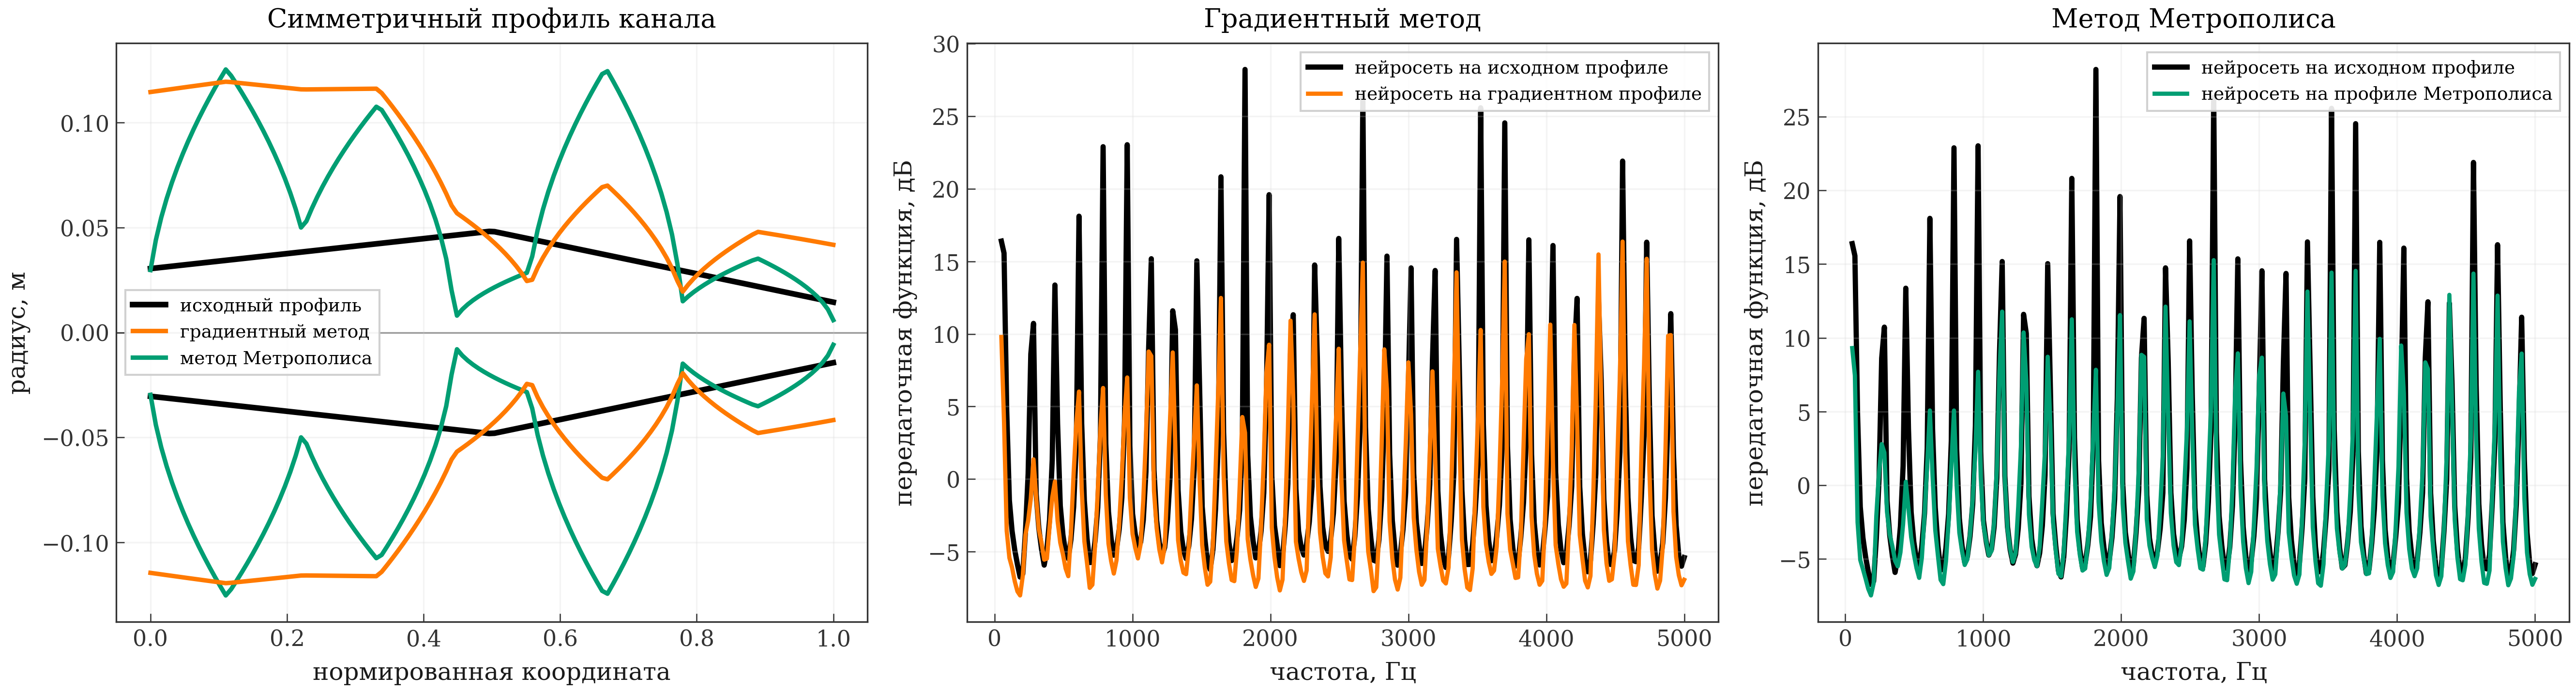
\includegraphics[width=0.95\textwidth]{images/обратная_задача_сравнение_методов.png}
    \caption{Сравнение результатов восстановления геометрии волновода и соответствующих АЧХ с помощью градиентного спуска и метода Метрополиса.}
    \label{fig:inverse_opt_comparison}
\end{figure}

Как видно из графиков геометрии (слева на рис.~\ref{fig:inverse_opt_comparison}), оба метода предсказывают довольно плохую форму исходного канала (наблюдаются сильные отклонения от истинного профиля площадей), что подтверждает неединственность решения обратной задачи. Однако при анализе соответствующих АЧХ (справа на рис.~\ref{fig:inverse_opt_comparison}) видно, что метод Метрополиса обеспечивает значительно более точную аппроксимацию спектрального отклика. В частности, метод Метрополиса дает более или менее правильные нижние границы $H$ (положение и глубину провалов АЧХ), тогда как градиентный спуск застревает в локальных минимумах и не может восстановить антирезонансы.

\subsection{Глубокое обучение: UNet на картах [H, f, x]}
\label{subsec:unet_inverse}

Для преодоления ограничений традиционной оптимизации был разработан метод на основе сверточной нейросети UNet (\text{TransferMapInverseUNet}). Поскольку стандартный спектральный отклик является одномерным вектором $H(f) \in \mathbb{R}^{N_f}$, а геометрия имеет пространственную размерность $A(x) \in \mathbb{R}^{N_s}$, для применения 2D-сверток одномерная АЧХ преобразуется в 2D пространственно-спектральную карту входа размерности $[C, N_f, N_s]$.

Были исследованы два режима формирования входной карты (рис.~\ref{fig:unet_input_map}):
\begin{itemize}
    \item \textbf{Режим трансляции (Broadcast)}: одномерная целевая АЧХ дублируется вдоль всей пространственной оси $x$, формируя однородную сетку.
    \item \textbf{Режим префиксного решателя (Prefix Solver)}: каждый столбец $j$ входной карты содержит АЧХ усеченной геометрии $[0, x_j]$, что позволяет физически связать частотный отклик с координатой распространения волны.
\end{itemize}

Входной тензор имеет три канала ($C=3$), содержащих значения АЧХ $H_{\mathrm{dB}}(f)$, нормированные частоты $f$ и нормированные пространственные координаты $x$.

\begin{figure}[H]
    \centering
    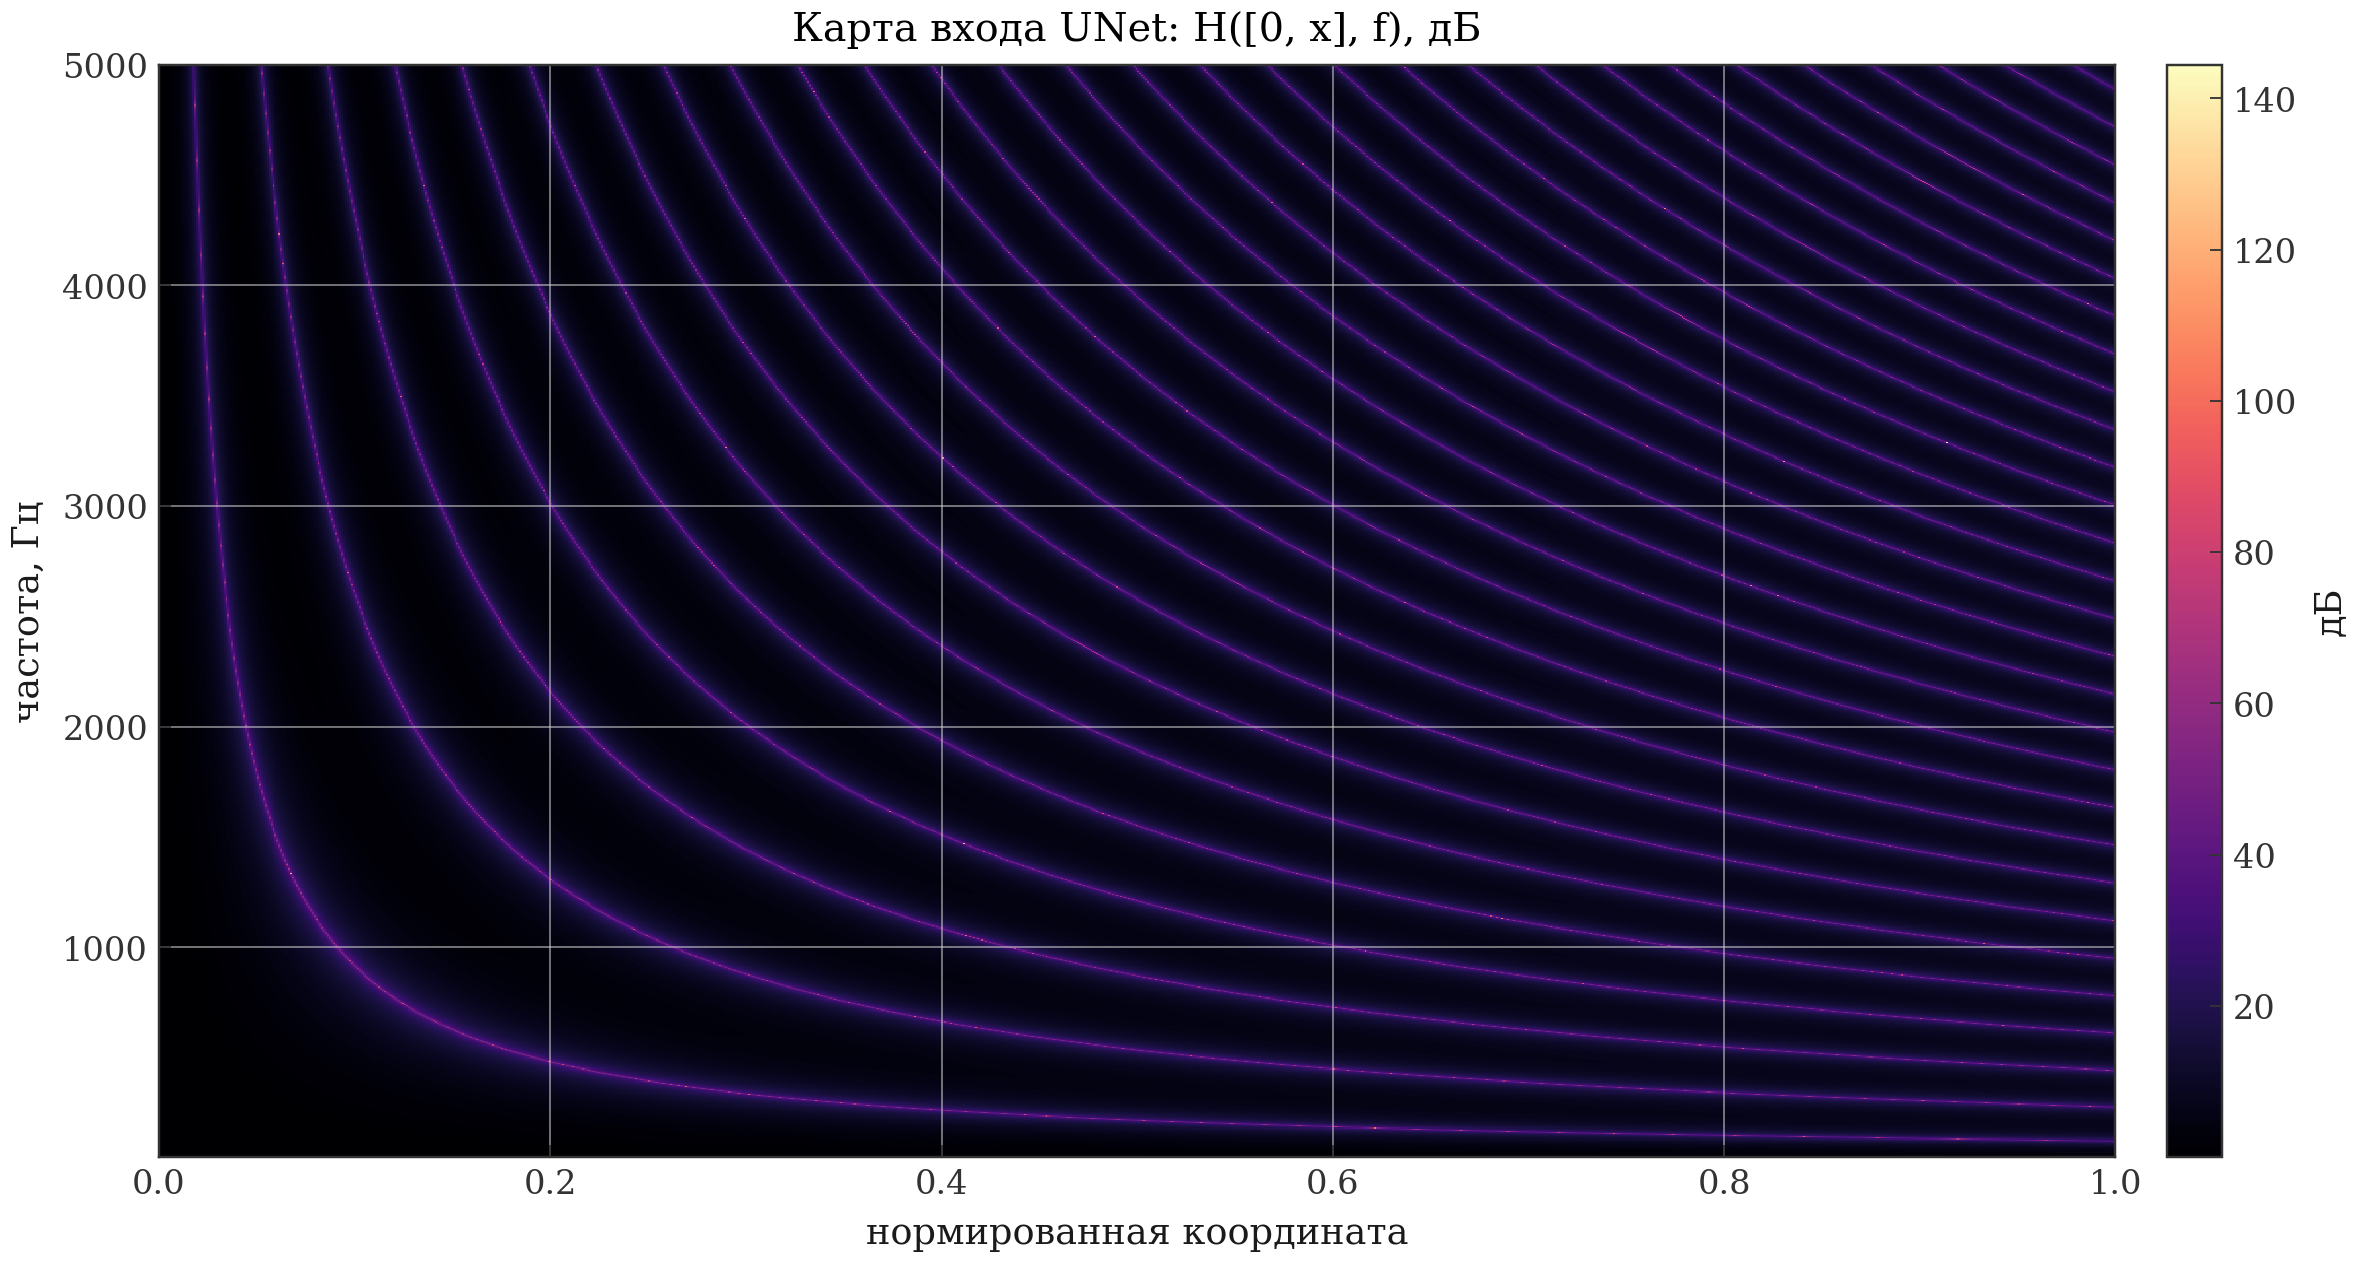
\includegraphics[width=0.85\textwidth]{images/обратная_задача_суперкарта.png}
    \caption{Пример двумерной входной пространственно-спектральной карты $[H, f, x]$ (суперкарты) высокого разрешения для сверточной модели UNet.}
    \label{fig:unet_input_map}
\end{figure}

Сверточная модель UNet обучается предсказывать 1D геометрический профиль волновода $A(x)$ по 2D входной карте. На рис.~\ref{fig:unet_input_maps_four} представлены двумерные входные пространственно-спектральные карты для четырех тестовых образцов волноводов, а результаты восстановления площадей сечений для них показаны на рис.~\ref{fig:unet_reconstructions}.

\begin{figure}[H]
    \centering
    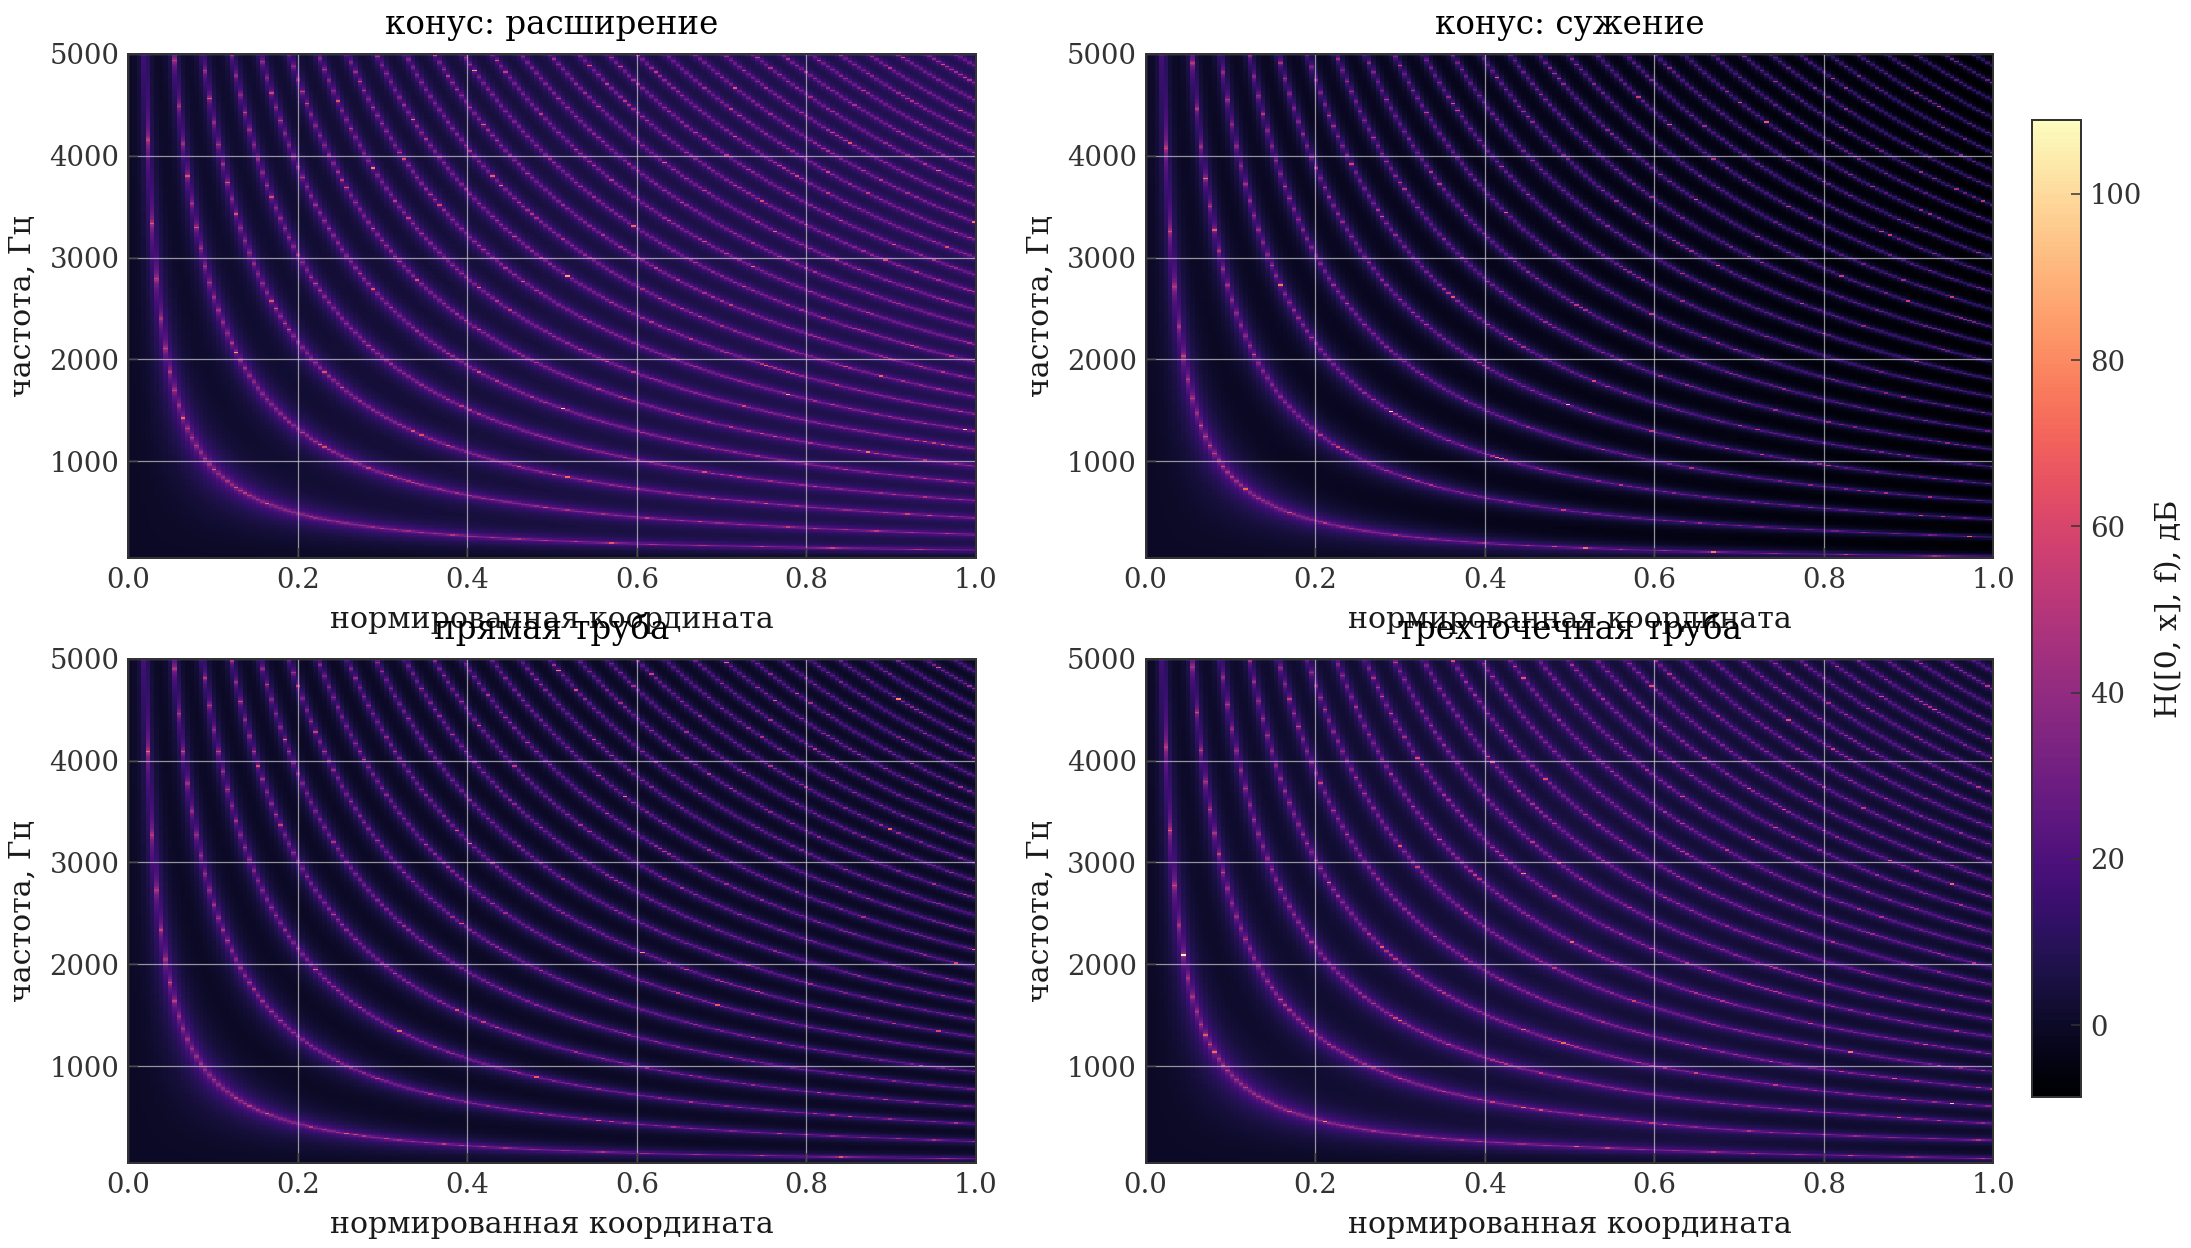
\includegraphics[width=0.95\textwidth]{images/обратная_задача_карты_к_трубам.png}
    \caption{Двумерные входные карты $[H, f, x]$ для четырех тестовых волноводов, используемые моделью UNet.}
    \label{fig:unet_input_maps_four}
\end{figure}

\begin{figure}[H]
    \centering
    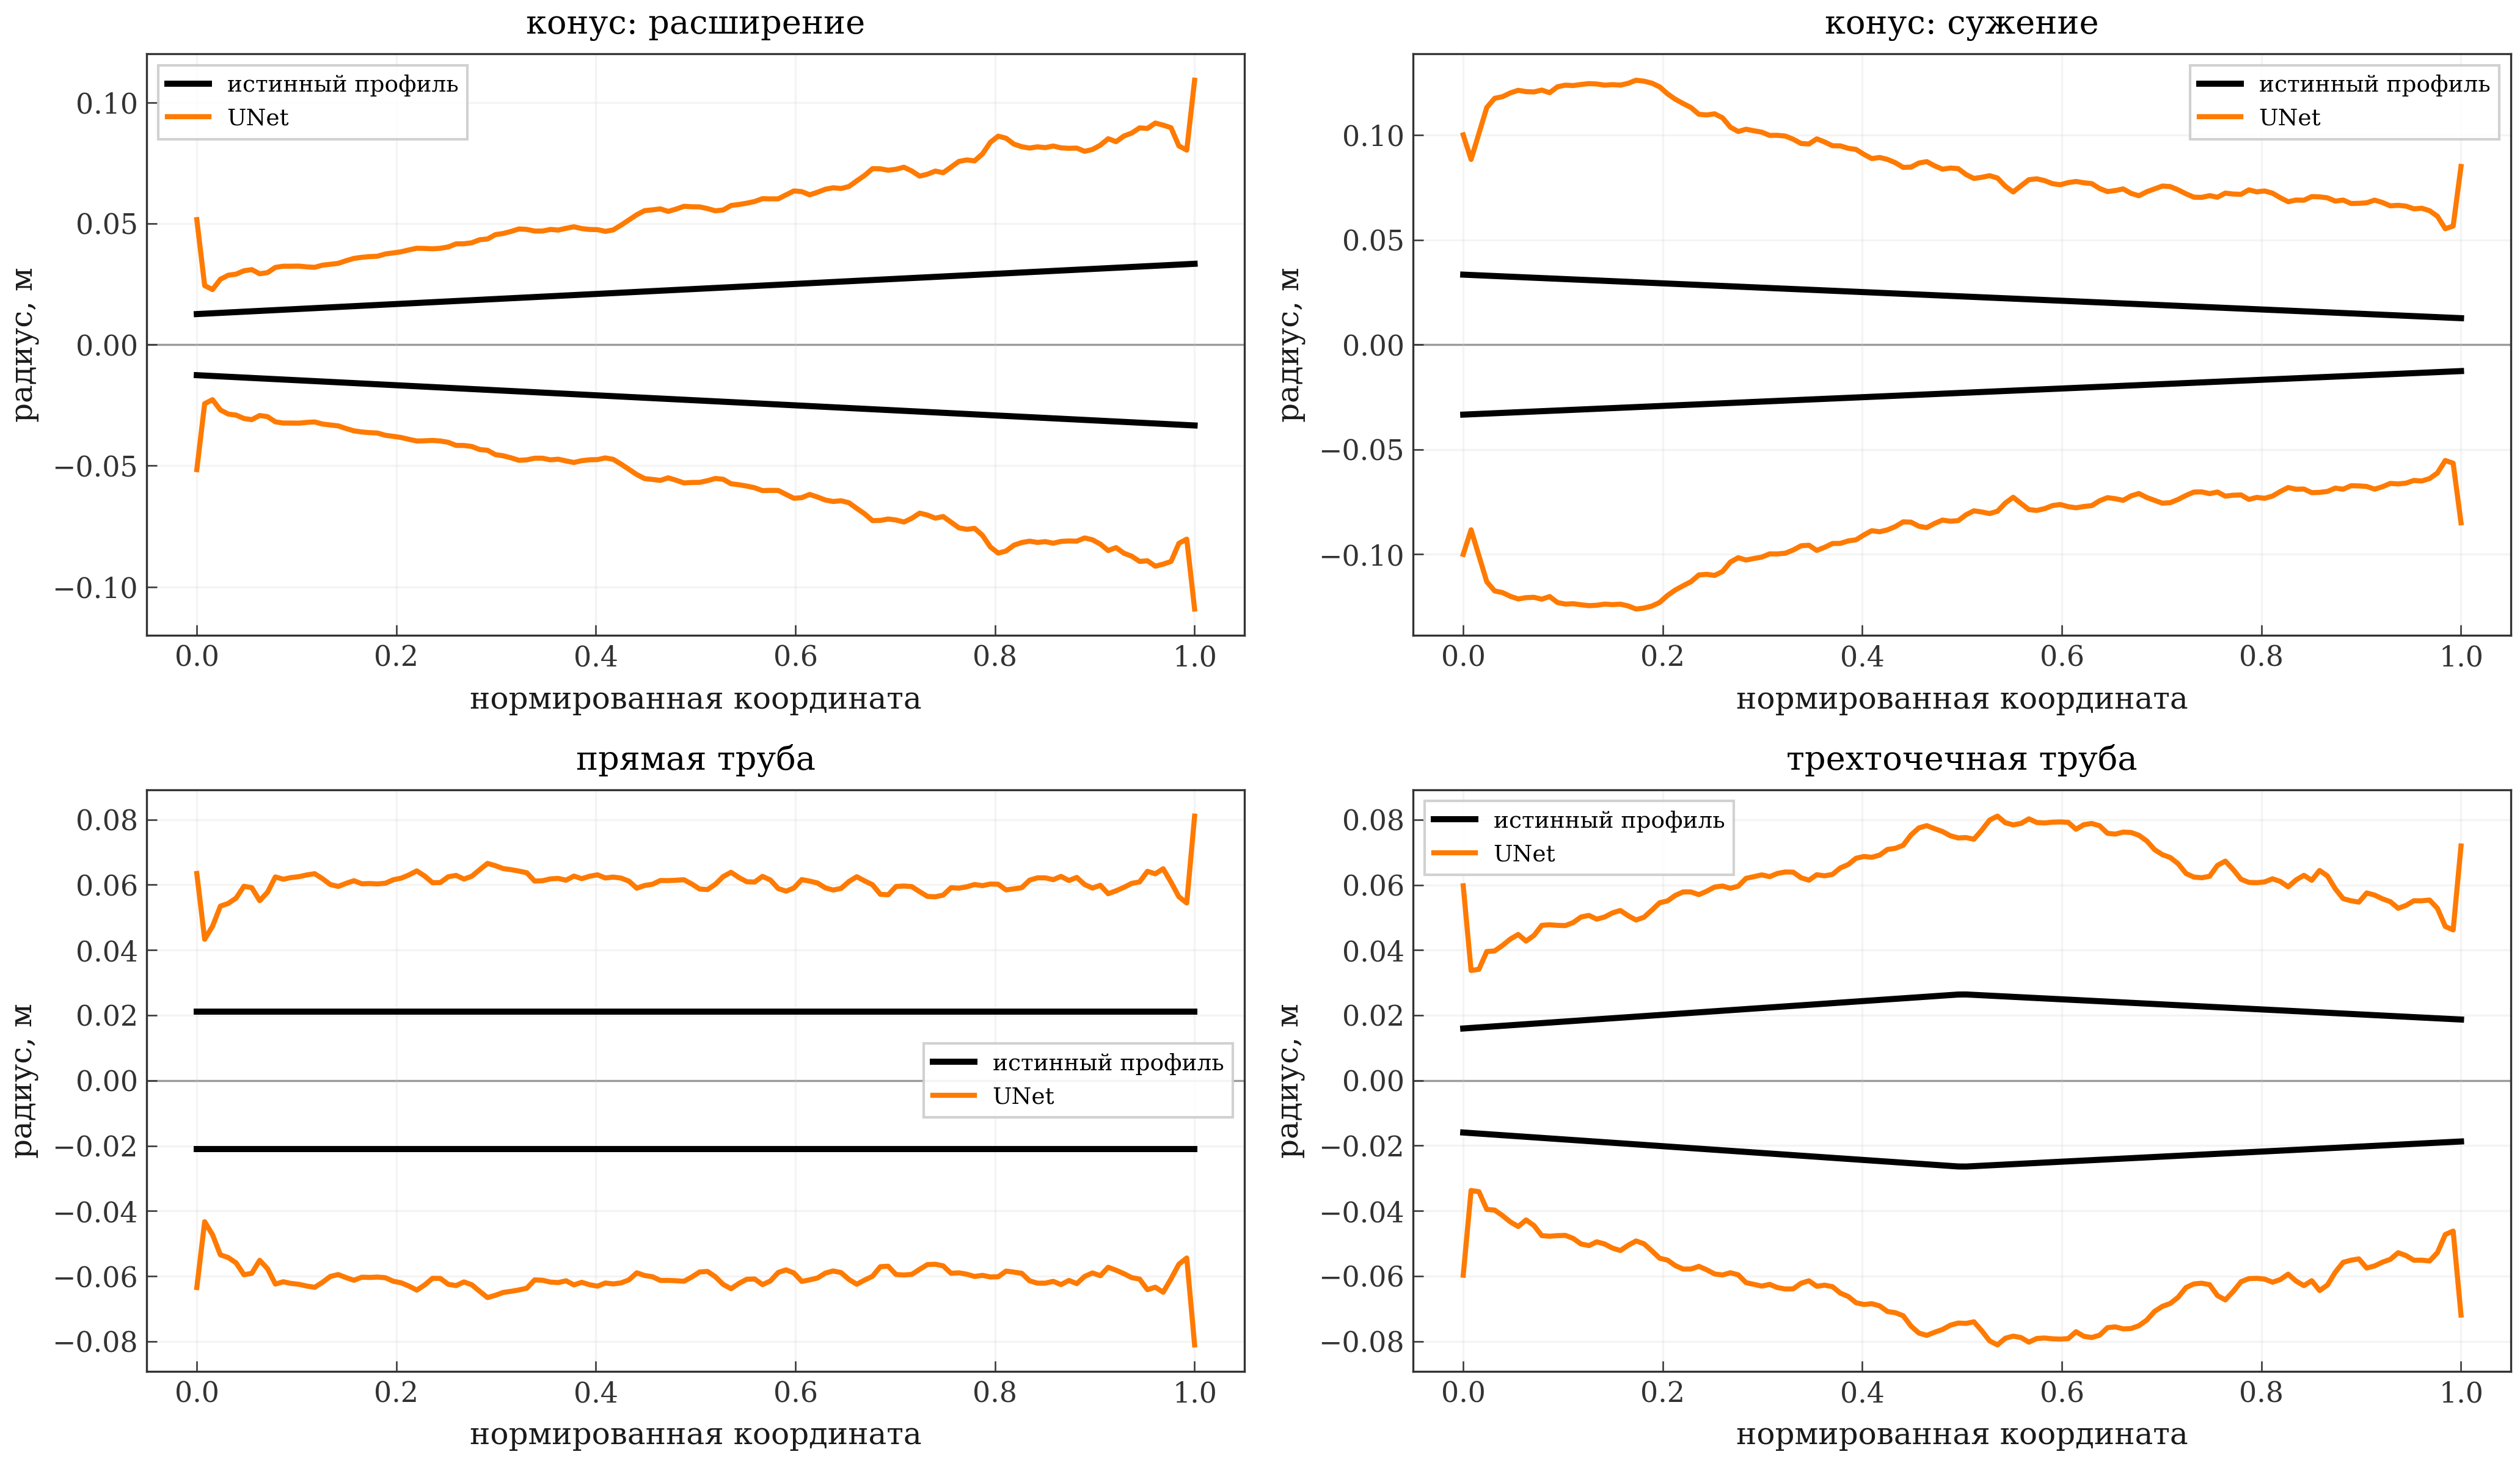
\includegraphics[width=0.95\textwidth]{images/обратная_задача_unet_четыре_геометрии.png}
    \caption{Примеры восстановления геометрических профилей четырех различных тестовых волноводов с помощью обученной сверточной модели UNet.}
    \label{fig:unet_reconstructions}
    \label{fig_count} % Для подсчета рисунков в аннотации
\end{figure}


% 6. Заключение
\chapter*{Заключение}
\addcontentsline{toc}{chapter}{Заключение}

В ходе выполнения первого этапа выпускной квалификационной работы бакалавра были успешно решены все поставленные задачи и получены следующие основные результаты:

\begin{enumerate}
    \item Проведен подробный анализ физико-математических основ одномерной акустики в волноводах переменного сечения на основе уравнения рупора Вебстера и граничных условий.
    \item Разработан и программно реализован в виде единого Python/C++ комплекса набор численных решателей, включающий:
    \begin{itemize}
        \item метод матриц передачи (TMM) для кусочно-цилиндрической и кусочно-конической аппроксимаций геометрии волновода;
        \item авторегрессионный z-доменный метод моделирования (ARMA);
        \item метод матриц длинных линий (TLM) во временной области в цилиндрической формулировке на C++.
    \end{itemize}
    \item На тестовых задачах регулярных форм (цилиндр, конус) проведена верификация численных схем, показавшая высокую точность расчетов и полное физическое соответствие.
    \item Исследовано качество геометрической аппроксимации волновода. Установлено, что коническая дискретизация обеспечивает меньшую относительную ошибку площади сечения по сравнению со ступенчатой цилиндрической при одинаковом числе разбиений.
    \item Выполнен сравнительный анализ точности расчета передаточных функций. Выявлено преимущество конического TMM-решателя для гладких геометрий, а также высокая точность быстрого авторегрессионного решателя (ARMA).
    \item Выполнена сравнительная оценка вычислительной производительности реализованных алгоритмов. Частотные методы (TMM, ARMA) показали наилучшую скорость расчетов на индивидуальных геометриях по сравнению с временным методом TLM.
\end{enumerate}

Полученные результаты и разработанный программный комплекс численных решателей могут служить основой для быстрого моделирования и массовой генерации данных в задачах одномерного акустического анализа. В качестве перспектив развития работы планируется интеграция реализованных физических решателей с нейросетевыми операторными моделями (FNO) для ускорения решения прямой задачи и оптимизационными методами для решения обратной задачи восстановления геометрии.


% 7. Список литературы
\newpage
\addcontentsline{toc}{chapter}{Список литературы}
\bibliographystyle{unsrt}
\bibliography{bibliography}
\label{ref_count} % Для подсчета источников в аннотации

\end{document}